\chapter{Thực nghiệm và Đánh giá}
\label{chap:experiment}

Chương này trình bày chi tiết về quá trình thực nghiệm nhằm kiểm chứng hiệu quả của mô hình đề xuất Two-Tower Multi-modal Recommendation System. Mục tiêu của các thực nghiệm là trả lời các câu hỏi nghiên cứu sau:

\begin{enumerate}
    \item Việc kết hợp đa phương thức bao gồm ``Văn bản'', ``Hình ảnh'', ``Dữ liệu bảng'' có cải thiện hiệu năng gợi ý so với đơn phương thức hay không?
    \item Mô hình giải quyết bài toán dự đoán hành vi tiếp theo Next-Item Prediction và vấn đề Cold-start hiệu quả như thế nào?
    \item Cơ chế Hybrid Retrieval, kết hợp Query ngữ nghĩa và Personalization đóng góp ra sao vào trải nghiệm người dùng cuối?
    \item Mô hình đề xuất có khả năng triển khai trong môi trường thực tế đảm bảo yêu cầu về độ trễ thấp và tính tương tác thời gian thực hay không?
\end{enumerate}

Nội dung chương bao gồm mô tả tập dữ liệu, thiết lập môi trường thực nghiệm, định nghĩa các độ đo đánh giá, phân tích sâu các kết quả thu được và minh họa hệ thống triển khai thực tế.

\section{Mô tả tập dữ liệu}
\label{sec:data_desc}

\subsection{Tổng quan về nguồn dữ liệu}
Nghiên cứu này sử dụng tập dữ liệu \textbf{Amazon Reviews 2023}, một bộ dữ liệu quy chuẩn phổ biến trong cộng đồng nghiên cứu Hệ thống gợi ý. Cụ thể, đồ án tập trung vào phân loại hàng hóa \textit{Gift Cards}. Đây là miền dữ liệu đặc thù với tính chất sản phẩm ít biến động về cấu hình kỹ thuật nhưng phụ thuộc nhiều vào ngữ cảnh tặng quà, hình ảnh minh họa và ý định của người mua.\\

Cấu trúc dữ liệu của hệ thống được tổ chức một cách khoa học thông qua hai tập tin định dạng JSON Lines riêng biệt. Mặc dù được lưu trữ tách rời để thuận tiện cho quá trình xử lý, hai tập tin này vẫn duy trì mối liên kết logic chặt chẽ nhằm đảm bảo tính toàn vẹn của thông tin. Cụ thể, tập tin \textbf{User Reviews} đóng vai trò trung tâm trong việc lưu trữ dữ liệu người dùng, bao gồm toàn bộ lịch sử tương tác, các nội dung phản hồi đánh giá cũng như mô hình hành vi chi tiết. Song song với đó, tập tin \textbf{Item Metadata} bổ trợ bằng cách cung cấp cơ sở dữ liệu chuyên sâu về sản phẩm, bao gồm các thông tin mô tả chi tiết và dữ liệu đa phương thức, giúp định danh và làm rõ ngữ cảnh cho các đối tượng được tương tác.\\

Dưới đây là phân tích chi tiết từng trường dữ liệu được sử dụng trong quá trình huấn luyện và kiểm thử mô hình.\\

\subsubsection*{A. Chi tiết dữ liệu User Reviews}
Tập dữ liệu này đóng vai trò là nguồn ``Ground Truth'' để mô hình học sở thích của người dùng. Mỗi dòng dữ liệu đại diện cho một lần tương tác cụ thể.

\begin{table}[H]
    \centering
    \caption{Mô tả chi tiết các trường thông tin trong tập dữ liệu User Reviews}
    \label{tab:user_reviews_desc}
    \renewcommand{\arraystretch}{1.3} % Tăng khoảng cách dòng cho dễ đọc
    \begin{tabular}{|p{0.25\linewidth}|p{0.7\linewidth}|}
        \hline
        \textbf{Trường dữ liệu} & \textbf{Mô tả và Phương pháp xử lý} \\
        \hline
        \texttt{user\_id} \newline \textit{(String)} & 
        Định danh duy nhất của người dùng. Đây là khóa chính để gom nhóm lịch sử hành vi. Toàn bộ tương tác của cùng một \texttt{user\_id} được sắp xếp theo thời gian để làm đầu vào cho User Tower. \\
        \hline
        \texttt{parent\_asin} \newline \textit{(String)} & 
        Mã định danh cha của sản phẩm, đại diện cho nhóm các biến thể màu sắc và kiểu dáng. Đồ án sử dụng trường này làm khóa ngoại liên kết với Metadata nhằm giảm độ thưa dữ liệu. \\
        \hline
        \texttt{rating} \newline \textit{(Float)} & 
        Điểm đánh giá đại diện cho tín hiệu phản hồi hiện trần. Các tương tác có $\texttt{rating} \ge 4.0$ được xem là tích cực. Giá trị này cũng được dùng làm đặc trưng số học cho Tabular Encoder. \\
        \hline
        \texttt{title} \& \texttt{text} \newline \textit{(String)} & 
        \texttt{title} tóm tắt cảm xúc chính, còn \texttt{text} chứa nội dung chi tiết phản ánh lý do mua hàng. Hai trường này được nối lại thành chuỗi văn bản đầu vào cho Text Encoder. \\
        \hline
        \texttt{timestamp} \newline \textit{(Integer)} & 
        Thời gian đánh giá. Dữ liệu được sắp xếp tăng dần theo trường này để mô phỏng đúng bài toán \textit{Sequential Recommendation}, tránh rò rỉ dữ liệu tương lai. \\
        \hline
        \texttt{verified\_purchase} \newline \textit{(Boolean)} & 
        Nhãn xác thực việc mua hàng. Được mã hóa thành Embedding trong Tabular Encoder để giúp mô hình phân biệt độ tin cậy giữa tương tác thật và ảo. \\
        \hline
        \texttt{helpful\_vote} \newline \textit{(Integer)} & 
        Số lượng người khác thấy bài review hữu ích. Giá trị này được chuẩn hóa Log normalization và đưa vào mô hình như một chỉ số đo lường chất lượng tương tác. \\
        \hline
    \end{tabular}
\end{table}

\subsubsection*{B. Chi tiết dữ liệu Item Metadata}
Tập dữ liệu này cung cấp các đặc trưng nội dung để xây dựng Item Tower đa phương thức.

\begin{table}[H]
    \centering
    \caption{Mô tả chi tiết các trường thông tin trong tập dữ liệu Item Metadata}
    \label{tab:item_metadata_desc}
    \renewcommand{\arraystretch}{1.3} % Tăng khoảng cách dòng
    \begin{tabular}{|p{0.3\linewidth}|p{0.65\linewidth}|}
        \hline
        \textbf{Trường dữ liệu} & \textbf{Mô tả và Phương pháp xử lý} \\
        \hline
        \texttt{parent\_asin} \newline \textit{(String)} & 
        Khóa chính của sản phẩm. Được dùng để ánh xạ 1-nhiều với dữ liệu trong bảng User Reviews. \\
        \hline
        \texttt{title} \newline \textit{(String)} & 
        Tên đầy đủ của sản phẩm, chứa thông tin thương hiệu, mệnh giá và dịp tặng quà. Đây là đặc trưng quan trọng nhất, được mã hóa bởi BERT/MPNet để tạo vector ngữ nghĩa. \\
        \hline
        \texttt{images} \newline \textit{(List)} & 
        Danh sách ảnh sản phẩm gồm \texttt{thumb}, \texttt{large} và \texttt{hi\_res}. Ảnh chất lượng cao gồm (\texttt{hi\_res/large}) được tải về và đưa qua Vision Transformer để trích xuất đặc trưng thị giác. \\
        \hline
        \texttt{main\_category} \newline \textit{(String)} & 
        Danh mục chính (ví dụ: ``Gift Cards''). Giúp định danh miền dữ liệu. Được xử lý bằng One-hot hoặc Embedding cho Tabular Encoder. \\
        \hline
        \texttt{categories} \newline \textit{(List)} & 
        Phân cấp sản phẩm. Được xử lý để tạo embedding đại diện nhóm hàng, giúp mô hình gom cụm các sản phẩm tương đồng. \\
        \hline
        \texttt{store} \newline \textit{(String)} & 
        Thương hiệu phát hành thẻ (ví dụ: Amazon, Visa). Đây là đặc trưng định danh quan trọng, được chuyển đổi thành chỉ số Index và đưa qua lớp Embedding. \\
        \hline
        \texttt{avg\_rating} \textit{(Float)} \& \newline \texttt{rating\_number} \textit{(Int)} & 
        Điểm trung bình và tổng lượt đánh giá - các chỉ số ``Bằng chứng xã hội''. Dữ liệu này được chuẩn hóa để tránh chênh lệch thang đo khi đưa vào mạng nơ-ron. \\
        \hline
        \texttt{price} \newline \textit{(Float)} & 
        Giá bán (USD). Cung cấp thông tin phân khúc giá trị. Các giá trị thiếu được xử lý bằng phương pháp gán trung vị. \\
        \hline
        \texttt{features}, \texttt{description} \newline \& \texttt{details} & 
        Các mô tả bổ sung và thông số kỹ thuật dạng key-value. Chúng bổ sung ngữ nghĩa cho tiêu đề và được chuyển đổi thành văn bản để bổ trợ cho Text Encoder. \\
        \hline
    \end{tabular}
\end{table}

\subsubsection*{C. Mối quan hệ và Thách thức dữ liệu}
\textbf{Mối quan hệ liên kết:} Dữ liệu được liên kết thông qua trường \texttt{parent\_asin}. Quá trình tiền xử lý thực hiện phép nối Inner Join giữa Review và Metadata. Chỉ những cặp $(u, i)$ mà trong đó sản phẩm $i$ có đầy đủ thông tin, đặc biệt là ảnh và tiêu đề mới được giữ lại để huấn luyện.

\textbf{Thách thức:}Quá trình xử lý dữ liệu đối mặt với hai thách thức chính. Đầu tiên là sự \textit{đa dạng định dạng}, khi tập dữ liệu bao gồm hỗn hợp văn bản phi cấu trúc, hình ảnh, dữ liệu số và danh mục. Sự không đồng nhất này đòi hỏi kiến trúc mạng nơ-ron phải đủ phức tạp để thực hiện fusion hiệu quả các nguồn tin đa phương thức. Thách thức thứ hai đến từ \textit{nhiễu dữ liệu}, biểu hiện qua việc thiếu hụt hình ảnh, ảnh chất lượng thấp hoặc các đánh giá ngắn, thiếu ngữ nghĩa. Do đó, quy trình tiền xử lý và làm sạch dữ liệu đóng vai trò then chốt để đảm bảo chất lượng đầu vào cho mô hình.

\subsection{Phân tích chất lượng dữ liệu và Giá trị khuyết}
\label{sec:missing_data}

Để đảm bảo tính tin cậy của đầu vào mô hình, chúng tôi đã thực hiện thống kê chi tiết tỷ lệ dữ liệu khuyết trên cả hai tập dữ liệu chính: Thông tin sản phẩm và Tương tác người dùng.

\subsubsection*{A. Đối với Dữ liệu sản phẩm}
Kết quả thống kê trên tổng số \textbf{1,137} sản phẩm cho thấy sự phân hóa rõ rệt về chất lượng giữa các trường thông tin.

\begin{table}[H]
    \centering
    \caption{Thống kê tỷ lệ dữ liệu khuyết trên Item Metadata}
    \label{tab:missing_meta}
    \renewcommand{\arraystretch}{1.3} % Tăng giãn dòng giống bảng trên
    \setlength{\tabcolsep}{5pt} % Căn chỉnh khoảng cách cột
    \begin{tabular}{|p{0.25\linewidth}|c|c|p{0.35\linewidth}|}
        \hline
        \textbf{Thuộc tính} & \textbf{SL Thiếu} & \textbf{Tỷ lệ (\%)} & \textbf{Phương án xử lý} \\
        \hline
        Title & 0 & 0.00\% & Giữ nguyên. \\
        \hline
        Average Rating & 0 & 0.00\% & Sử dụng trực tiếp. \\
        \hline
        Images & 1 & 0.09\% & Loại bỏ sản phẩm hoặc dùng ảnh mặc định. \\
        \hline
        Store & 17 & 1.50\% & Gán nhãn ``Unknown''. \\
        \hline
        Features & 105 & 9.23\% & Thay thế bằng chuỗi rỗng. \\
        \hline
        Main Category & 170 & 14.95\% & Gán nhãn danh mục chung hoặc ``Gift Cards''. \\
        \hline
        Description & 262 & 23.04\% & Thay thế bằng chuỗi rỗng, tập trung vào Title. \\
        \hline
        Price & 757 & 66.58\% & Gán giá trị trung vị (Median Imputation). \\
        \hline
        Videos/Subtitle & 1137 & 100.00\% & Loại bỏ trường dữ liệu. \\
        \hline
    \end{tabular}
\end{table}

\textbf{Nhận xét và Chiến lược xử lý:}\\

Dựa trên kết quả thống kê, đồ án đề xuất chiến lược xử lý dữ liệu tập trung vào hai khía cạnh chính:\\

Đầu tiên, đối với biến \textbf{Giá}, tỷ lệ khuyết dữ liệu lên tới 66.58\% phản ánh đặc thù mệnh giá động của loại hình Gift Card. Thay vì loại bỏ trường thông tin quan trọng này, nghiên cứu áp dụng phương pháp \textit{Gán giá trị trung vị}. Phương pháp này giúp duy trì thông tin về phân khúc giá trị sản phẩm đồng thời hạn chế tác động của các giá trị ngoại lai. Tuy nhiên, để đảm bảo tính ổn định, trọng số của nhánh Tabular Encoder sẽ được điều chỉnh giảm so với các nhánh xử lý văn bản và hình ảnh.\\

Thứ hai, đối với các trường thông tin không mang lại giá trị phân tích hoặc có tỷ lệ khuyết tuyệt đối 100\% như \texttt{bought\_together}, \texttt{subtitle} và \texttt{author}, chiến lược \textit{Cắt tỉa đặc trưng} được áp dụng triệt để. Việc loại bỏ các trường này không chỉ giúp làm sạch nhiễu mà còn tối ưu hóa tài nguyên bộ nhớ và không gian lưu trữ cho quá trình huấn luyện mô hình.

\subsubsection*{B. Đối với Dữ liệu tương tác}
Trái ngược với đặc điểm phân tán của tập Metadata, dữ liệu Reviews sau quá trình sàng lọc \textit{k-core filtering} thể hiện tính toàn vẹn và độ tin cậy cao. Kết quả thống kê cho thấy tập dữ liệu bao gồm \textbf{152,410} tương tác, với tỷ lệ dữ liệu khuyết là \textbf{0\%} trên tất cả các trường thông tin trọng yếu bao gômf \texttt{user\_id}, \texttt{parent\_asin}, \texttt{rating} và \texttt{timestamp}. 

Điều này đảm bảo rằng User Tower sẽ luôn nhận được đầu vào đầy đủ và nhất quán, không cần phải thực hiện các kỹ thuật điền khuyết phức tạp cho chuỗi hành vi, giúp quá trình huấn luyện mô hình tuần tự diễn ra ổn định.
\subsection{Quy trình Tiền xử lý dữ liệu}
\label{sec:preprocessing}


Do tính chất đa phương thức và độ nhiễu cao của dữ liệu thương mại điện tử thực tế, quy trình tiền xử lý đóng vai trò then chốt trong việc đảm bảo tính hội tụ và hiệu năng của mô hình. Quy trình này được chia thành 4 giai đoạn chính: Làm sạch dữ liệu, Xử lý đặc trưng đa phương thức, Chuẩn hóa dữ liệu bảng và Xây dựng chuỗi hành vi tuần tự.

\subsubsection*{Giai đoạn 1: Làm sạch và Lọc dữ liệu}
Dữ liệu thô thu thập từ Amazon thường chứa nhiều giá trị bị khuyết và các điểm dữ liệu nhiễu. Quy trình tiền xử lý dữ liệu được tiến hành qua hai giai đoạn trọng tâm nhằm chuẩn hóa đầu vào cho mô hình, các bước xử lý bao gồm:\\

Giai đoạn thứ nhất tập trung vào \textbf{xử lý giá trị khuyết} với các chiến lược riêng biệt cho từng loại dữ liệu. Cụ thể, các mẫu thiếu trường định danh cốt lõi như \texttt{title} sẽ bị loại bỏ hoàn toàn để đảm bảo tính nhất quán. Đối với dữ liệu số học như \texttt{price}, phương pháp gán giá trị trung vị được ưu tiên áp dụng thay vì giá trị trung bình, giúp giảm thiểu tác động lệch chuẩn gây ra bởi các giá trị ngoại lai. Trong khi đó, các giá trị rỗng tại các trường văn bản bổ trợ như \texttt{features} hay \texttt{description} được xử lý bằng cách điền thế chuỗi ký tự trống ``'' để đảm bảo tính hợp lệ kỹ thuật cho bộ mã hóa.\\

Giai đoạn thứ hai là \textbf{sàng lọc tương tác}, áp dụng kỹ thuật \textit{k-core filtering} với ngưỡng $k=3$ nhằm tối ưu hóa dữ liệu cho bài toán \textit{Sequential Recommendation}. Về phía người dùng, hệ thống loại bỏ các tài khoản có dưới 3 tương tác, Cold-start Users, do nhóm này không cung cấp đủ độ dài chuỗi lịch sử cần thiết để mô hình Transformer học được các mẫu hành vi phụ thuộc. Song song với đó, các sản phẩm có tần suất xuất hiện quá thấp, dưới 2 lần, cũng được lược bỏ để đảm bảo không gian biểu diễn được học từ dữ liệu đủ dày đặc.

\subsubsection*{Giai đoạn 2: Xử lý đặc trưng phi cấu trúc}
Đây là bước chuẩn bị đầu vào cho hai nhánh mạng nơ-ron chính: Text Encoder và Image Encoder.

\textbf{1. Xử lý dữ liệu văn bản:} \\
Do thông tin ngữ nghĩa của sản phẩm nằm rải rác ở nhiều trường khác nhau, chúng tôi thực hiện chiến lược nối chuỗi:
\begin{equation}
    \text{Text}_{input} = [\text{Title}] \oplus [\text{Description}] \oplus [\text{Features}] \oplus [\text{Details}]
\end{equation}
Trong đó $\oplus$ là phép nối chuỗi kèm theo ký tự phân cách đặc biệt. Chuỗi văn bản tổng hợp này sau đó được đưa qua bộ phân tách từ của mô hình \texttt{all-mpnet-base-v2}. Quá trình Tokenization tuân thủ các quy tắc:
\begin{itemize}
    \item \textbf{Padding:} Các chuỗi ngắn hơn độ dài tối đasẽ được thêm token \texttt{[PAD]} để đảm bảo kích thước batch đồng nhất.
    \item \textbf{Truncation:} Các chuỗi quá dài sẽ bị cắt bớt để phù hợp với giới hạn đầu vào của BERT, thường là 512 tokens, ưu tiên giữ lại phần đầu của văn bản vì chứa thông tin quan trọng nhất.
\end{itemize}

\textbf{2. Xử lý dữ liệu hình ảnh:} \\
Dữ liệu ảnh được tải về từ các đường dẫn URL trong Metadata. Quy trình xử lý ảnh tuân theo chuẩn đầu vào của mô hình Vision Transformer:
\begin{itemize}
    \item \textbf{Tải và Lọc lỗi:} Sử dụng Multi-threading để tải ảnh. Các ảnh bị lỗi định dạng hoặc không thể tải sẽ bị loại bỏ hoặc thay thế bằng ảnh placeholder màu đen.
    \item \textbf{Resize \& Center Crop:} Ảnh được thay đổi kích thước về độ phân giải $224 \times 224$ pixels.
    \item \textbf{Chuẩn hóa:} Các giá trị pixel trong khoảng $[0, 255]$ được chuyển về khoảng $[0, 1]$ và sau đó được chuẩn hóa theo phân bố của tập dữ liệu ImageNet:
    \begin{equation}
        x_{norm} = \frac{x - \mu_{ImageNet}}{\sigma_{ImageNet}}
    \end{equation}
    Với $\mu = [0.485, 0.456, 0.406]$ và $\sigma = [0.229, 0.224, 0.225]$. Bước này giúp mô hình ViT pretrained hoạt động hiệu quả nhất.
\end{itemize}

\subsubsection*{Giai đoạn 3: Xử lý dữ liệu bảng}
Dữ liệu có cấu trúc bao gồm các biến phân loại và biến số được xử lý riêng biệt.\\

\textbf{1. Biến phân loại (\texttt{main\_category}, \texttt{store}):}
    Được chuyển đổi sang dạng số nguyên (Integer Mapping) thông qua kỹ thuật Label Encoding. Một từ điển (Vocabulary) được xây dựng để ánh xạ mỗi giá trị duy nhất (ví dụ: ``Starbucks'') sang một chỉ số ID (ví dụ: 124). Các giá trị mới xuất hiện trong tập Test sẽ được gán về token đặc biệt \texttt{<UNK>}.\\
    
\textbf{2. Biến danh sách phân loại (\texttt{categories}):}
    Một sản phẩm có thể thuộc nhiều danh mục con (ví dụ: [Gift Cards, Birthday, For Her]). Chúng tôi sử dụng phương pháp \textit{Multi-hot Encoding} kết hợp với \textit{Embedding Pooling}. Cụ thể, các ID của danh mục sẽ được tra cứu trong bảng Embedding, sau đó lấy trung bình (Average Pooling) để tạo ra một vector đại diện duy nhất cho trường này.\\
    
\textbf{3. Biến số (\texttt{rating}, \texttt{vote}, \texttt{price}):}
    Để giúp mạng nơ-ron hội tụ nhanh hơn, các biến số được chuẩn hóa bằng \textit{Standard Scaler} (Z-score normalization):
    \begin{equation}
        z = \frac{x - \mu}{\sigma}
    \end{equation}
    Riêng đối với biến \texttt{helpful\_vote}, do phân bố lệch trái nặng (phần lớn là 0 hoặc số nhỏ), chúng tôi áp dụng biến đổi Logarit trước khi chuẩn hóa: $x' = \log(1 + x)$.

\subsubsection*{Giai đoạn 4: Xây dựng chuỗi tương tác}
Đây là bước quan trọng nhất để huấn luyện User Tower. Dữ liệu tương tác được gom nhóm theo \texttt{user\_id} và sắp xếp tăng dần theo \texttt{timestamp}.

Với mỗi người dùng $u$, ta có chuỗi hành vi $S_u = \{i_1, i_2, ..., i_T\}$. Quá trình tạo mẫu huấn luyện (Training Samples) được thực hiện theo cơ chế \textit{Sliding Window}:
\begin{itemize}
    \item Tại mỗi bước thời gian $t$ ($1 < t \le T$), mô hình sử dụng chuỗi lịch sử $H_t = \{i_1, ..., i_{t-1}\}$ để dự đoán item mục tiêu $i_t$.
    \item \textbf{Padding:} Nếu độ dài chuỗi lịch sử nhỏ hơn độ dài tối đa quy định ($L=40$), chúng tôi thêm các token \texttt{[PAD]} vào bên trái chuỗi.
    \item \textbf{Masking:} Một ma trận mặt nạ được tạo ra để báo cho lớp Self-Attention trong Transformer biết cần bỏ qua các vị trí là \texttt{[PAD]}, đảm bảo tính toán chỉ tập trung vào các tương tác thực tế.
\end{itemize}
Thống kê chi tiết được trình bày trong Bảng \ref{tab:dataset_stats}.

\begin{table}[H]
    \centering
    \caption{Thống kê tập dữ liệu Amazon Gift Cards sau khi tiền xử lý}
    \label{tab:dataset_stats}
    \renewcommand{\arraystretch}{1.3} % Tăng khoảng cách dòng
    \setlength{\tabcolsep}{5pt} % Căn chỉnh khoảng cách cột
    \begin{tabular}{|p{0.35\linewidth}|c|p{0.4\linewidth}|}
        \hline
        \textbf{Thông số} & \textbf{Số lượng} & \textbf{Mô tả} \\
        \hline
        Tổng số người dùng  & 73,929 & Số lượng người dùng duy nhất. \\
        \hline
        Tổng số sản phẩm & 1,137 & Số lượng thẻ quà tặng khác nhau. \\
        \hline
        Tổng số tương tác & 78,095 & Tổng số lượt review/rating hợp lệ. \\
        \hline
        Độ dài chuỗi trung bình & $\sim 1.06$ & Số lượng tương tác trung bình trên một người dùng. \\
        \hline
    \end{tabular}
\end{table}
Kết quả của quá trình tiền xử lý là các Tensor định dạng PyTorch sẵn sàng được đưa vào GPU để huấn luyện.

\subsection{Phân tích độ thưa dữ liệu}
\label{sec:sparsity_analysis}

\subsubsection*{A. Cơ sở lý thuyết và Định nghĩa}
Trong các hệ thống gợi ý, dữ liệu thường được biểu diễn dưới dạng một ma trận tương tác User-Item $R$ có kích thước $|U| \times |I|$, trong đó $|U|$ là tổng số người dùng và $|I|$ là tổng số sản phẩm. Mỗi phần tử $r_{ui}$ trong ma trận biểu thị tương tác của người dùng $u$ lên sản phẩm $i$.

Độ thưa phản ánh tỷ lệ các phần tử rỗng trong ma trận này. Một ma trận có độ thưa quá cao đồng nghĩa với việc thông tin hành vi người dùng cực kỳ hạn chế, gây khó khăn cho việc tìm kiếm các mẫu tương đồng. Độ thưa được định nghĩa bởi công thức \cite{31}:

\begin{equation}
    \text{Sparsity} = 1 - \text{Density} = 1 - \frac{\text{Total Interactions}}{|U| \times |I|}
\end{equation}

\subsubsection*{B. Tính toán thực nghiệm trên tập dữ liệu Amazon}
Dựa trên các thống kê đã trình bày ở Bảng \ref{tab:dataset_stats}, chúng tôi tiến hành tính toán độ thưa cụ thể cho tập dữ liệu huấn luyện:

\begin{itemize}
    \item Tổng số người dùng ($|U|$): $73,929$
    \item Tổng số sản phẩm ($|I|$): $1,137$
    \item Tổng số tương tác quan sát được ($N$): $78,095$
\end{itemize}

Kích thước không gian mẫu là:
$$ |U| \times |I| = 73,929 \times 1,137 \approx 84,057,273 $$

Mật độ dữ liệu thực tế:
$$ \text{Density} = \frac{78,095}{84,057,273} \approx 0.000929 \ ( 0.09\%) $$

Từ đó, độ thưa của tập dữ liệu là:
$$ \text{Sparsity} = 1 - 0.000929 \approx 0.999071 \ (\mathbf{99.91\%}) $$

\subsubsection*{C. Đánh giá và Tác động đến mô hình}
Kết quả tính toán $99.82\%$ cho thấy tập dữ liệu Amazon Gift Cards thuộc nhóm ``Extreme Sparsity''. Để so sánh, các tập dữ liệu chuẩn như MovieLens-1M thường có độ thưa khoảng $95-96\%$. Việc độ thưa tiệm cận $100\%$ đặt ra hai thách thức nghiêm trọng:\\


 Thứ nhất, \textbf{sự thất bại của Collaborative Filtering thuần túy:} Các thuật toán CF truyền thống như Matrix Factorization dựa vào việc tìm kiếm người dùng có hành vi tương đồng hoặc sản phẩm tương đồng thông qua sự chồng lấp các tương tác. Với mật độ $0.09\%$, xác suất để hai người dùng bất kỳ cùng đánh giá một sản phẩm là cực thấp, dẫn đến việc mô hình không thể tính toán độ tương đồng tin cậy.\\
    
Thứ hai, \textbf{vấn đề Cold-start:} Phần lớn người dùng trong tập dữ liệu chỉ có số lượng tương tác tối thiểu khoảng 2-3 tương tác. Mô hình không có đủ lịch sử hành vi để học được vector đại diện User Embedding chính xác nếu chỉ dựa vào ID.


\subsubsection*{D. Giải pháp tiếp cận: Content-based Multi-modal Learning}
Chính vì thách thức về độ thưa nêu trên, đồ án này bắt buộc phải chuyển hướng từ việc chỉ khai thác dữ liệu tương tác sang khai thác dữ liệu nội dung.

Cụ thể, kiến trúc Two-Tower được thiết kế để tận dụng các đặc trưng giàu ngữ nghĩa luôn có sẵn, bất kể người dùng đã tương tác hay chưa:
\begin{itemize}
    \item \textbf{Text Encoder (BERT):} Giúp mô hình hiểu rằng ``Visa Gift Card'' và ``Mastercard Gift Card'' là tương đồng về mặt ngữ nghĩa, ngay cả khi chưa có người dùng nào mua cả hai.
    \item \textbf{Image Encoder (ViT):} Giúp liên kết các sản phẩm có hình thức trình bày giống nhau (ví dụ: cùng chủ đề Giáng sinh, Sinh nhật) thông qua đặc trưng thị giác.
    \item \textbf{Tabular Encoder (MLP):} Xử lý các dữ liệu cấu trúc như \textit{Giá bán, Điểm đánh giá, Thương hiệu}. Nhánh này giúp mô hình học được các ngưỡng lọc quan trọng (ví dụ: người dùng chỉ thích mua thẻ mệnh giá thấp $<\$50$) để thu hẹp không gian tìm kiếm hiệu quả.
\end{itemize}

Nhờ cơ chế Fusion Gate kết hợp các thông tin này, mô hình có thể lấp đầy các khoảng trống trong ma trận thưa bằng các suy luận dựa trên nội dung, từ đó cải thiện đáng kể độ chính xác gợi ý như Recall hay NDCG sẽ được trình bày trong phần Kết quả thực nghiệm.

% [PLACEHOLDER CHO ẢNH]
% Bạn hãy thêm ảnh Histogram phân bố độ dài chuỗi hành vi của User vào đây
%\begin{figure}[H]
%%%    \centering
%%%    
\includegraphics[width=0.8\textwidth]{imagedothua.png} 
%%%    \caption{Phân bố độ dài chuỗi hành vi người dùng}
%%%    \label{fig:seq_dist}
%%%\end{figure}

\section{Thiết lập thực nghiệm}

\subsection{Môi trường phần cứng và phần mềm}
\subsubsection*{Cơ sở hạ tầng phần cứng}
Các thực nghiệm được triển khai trên nền tảng đám mây \textbf{Kaggle Kernels}, tận dụng sức mạnh tính toán hiệu năng cao của Google Cloud Platform (GCP). Việc sử dụng môi trường đám mây giúp giảm thiểu các sai số do sự khác biệt về phần cứng cá nhân và đảm bảo mô hình được huấn luyện trong điều kiện tối ưu.

Chi tiết cấu hình phần cứng như sau:

\begin{itemize}
    \item \textbf{Bộ xử lý đồ họa (GPU) :}
\begin{itemize}
        \item \textit{Loại thiết bị:} \textbf{NVIDIA Tesla P100-PCIE}.
        \item \textit{Kiến trúc:} Pascal.
        \item \textit{Bộ nhớ đồ họa (VRAM):} $16$ GB \textbf{HBM2}.
        \item \textit{Lý do lựa chọn:} Mặc dù là kiến trúc Pascal, Tesla P100 sở hữu băng thông bộ nhớ vượt trội ($\sim 732$ GB/s), cao hơn đáng kể so với các dòng GPU sử dụng bộ nhớ GDDR6 thông thường (như Tesla T4). Đặc điểm này cực kỳ tối ưu cho mô hình Two-Tower, nơi tác vụ Embedding Lookup cho hàng nghìn User/Item tiêu tốn tài nguyên băng thông rất lớn.
    \end{itemize}
    
    \item \textbf{Bộ xử lý trung tâm (CPU):}
    \begin{itemize}
        \item \textit{Cấu hình:} Intel(R) Xeon(R) CPU @ 2.20GHz (4 cores, 8 threads).
        \item \textit{Vai trò:} Chịu trách nhiệm cho các tác vụ tiền xử lý dữ liệu, tải ảnh đa luồng  và đưa dữ liệu vào hàng đợi trước khi đẩy sang GPU.
    \end{itemize}
    
    \item \textbf{Bộ nhớ trong (RAM):}
    \begin{itemize}
        \item \textit{Dung lượng:} $32$ GB System RAM.
        \item \textit{Vai trò:} Đảm bảo toàn bộ Meta-data và các vector đặc trưng sau khi trích xuất có thể được lưu trữ trên bộ nhớ đệm, tránh hiện tượng nghẽn cổ chai do đọc/ghi đĩa cứng liên tục.
    \end{itemize}
\end{itemize}

\subsubsection*{Hệ sinh thái phần mềm và Thư viện}
Mô hình được phát triển dựa trên ngôn ngữ lập trình \textbf{Python} phiên bản 3.10, ngôn ngữ tiêu chuẩn trong cộng đồng Trí tuệ nhân tạo hiện nay. Chúng tôi sử dụng các framework mã nguồn mở tiên tiến nhất để xây dựng kiến trúc mạng nơ-ron sâu.

Các thư viện chính bao gồm:

\begin{itemize}
    \item \textbf{PyTorch (v2.0+):} 
    Framework nền tảng cho Deep Learning. PyTorch được lựa chọn nhờ cơ chế đồ thị tính toán động, giúp linh hoạt trong việc xây dựng các kiến trúc phức tạp như Fusion Gate và tùy chỉnh hàm mất mát Contrastive Loss.
    
    \item \textbf{Hugging Face Transformers:} 
    Thư viện chuẩn mực cho các mô hình NLP. Chúng tôi sử dụng thư viện này để tải trọng số tiền huấn luyện của mô hình \texttt{all-mpnet-base-v2} và thực hiện quy trình Tokenization văn bản.
    
    \item \textbf{TIMM (PyTorch Image Models):} 
    Thư viện chuyên dụng cho các mô hình thị giác máy tính hiện đại. TIMM cung cấp kiến trúc \texttt{vit\_base\_patch16\_224} cùng các trọng số đã được huấn luyện trên ImageNet, giúp trích xuất đặc trưng ảnh chính xác mà không cần huấn luyện lại từ đầu.
    
    \item \textbf{Scikit-learn \& Pandas:} 
    Sử dụng cho các tác vụ xử lý dữ liệu bảng, phân chia tập dữ liệu, chuẩn hóa dữ liệu và tính toán các độ đo đánh giá cơ bản.
    
    \item \textbf{Các thư viện hỗ trợ khác:} 
    \begin{itemize}
        \item \texttt{tqdm}: Để theo dõi tiến độ huấn luyện trực quan.
        \item \texttt{matplotlib/seaborn}: Để trực quan hóa dữ liệu và biểu đồ Loss.
        \item \texttt{PIL (Pillow)}: Để xử lý và biến đổi dữ liệu ảnh thô.
    \end{itemize}
\end{itemize}


\subsection{Cấu hình Siêu tham số}
Quá trình huấn luyện được chia làm 2 giai đoạn: Huấn luyện Item Tower trước để tạo vector đặc trưng sản phẩm, sau đó dùng các vector này đóng băng hoặc tinh chỉnh nhẹ để huấn luyện User Tower.

\subsubsection*{Cấu hình Item Tower}
Item Tower chịu trách nhiệm mã hóa thông tin đa phương thức của sản phẩm. Các tham số chi tiết được liệt kê trong Bảng \ref{tab:item_params}.

\begin{table}[H]
    \centering
    \caption{Cấu hình siêu tham số cho Item Tower}
    \label{tab:item_params}
    \vspace{0.2cm}
    \begin{tabular}{l l p{6cm}}
        \toprule
        \textbf{Tham số} & \textbf{Giá trị} & \textbf{Giải thích} \\
        \midrule
        Text Encoder & \texttt{all-mpnet-base-v2} & Mô hình Sentence-BERT tối ưu cho Semantic Search \\
        Image Encoder & \texttt{vit\_base\_patch16\_224} & Vision Transformer pretrained trên ImageNet \\
        Batch Size & 128 & Kích thước lô dữ liệu \\
        Learning Rate & $2 \times 10^{-5}$ & Tốc độ học thấp để fine-tune \\
        Epochs & 70 & Số vòng lặp huấn luyện \\
        Temperature ($\tau$) & 0.07 & Tham số nhiệt độ cho Contrastive Loss \\
        Latent Dimension & 256 & Kích thước vector nhúng cuối cùng \\
        \bottomrule
    \end{tabular}
\end{table}

\subsubsection*{Cấu hình User Tower}
User Tower sử dụng kiến trúc Transformer Encoder để học sự phụ thuộc tuần tự trong lịch sử hành vi người dùng.

\begin{table}[H]
    \centering
    \caption{Cấu hình siêu tham số cho User Tower}
    \label{tab:user_params}
    \vspace{0.2cm}
    \begin{tabular}{l l p{6cm}}
        \toprule
        \textbf{Tham số} & \textbf{Giá trị} & \textbf{Giải thích} \\
        \midrule
        Architecture & Transformer Encoder & Sử dụng Self-Attention \\
        Num Layers & 2 & Số lớp Transformer \\
        Num Heads & 4 & Số đầu Attention \\
        Max Seq Length & 40 & Độ dài chuỗi lịch sử tối đa \\
        LR (Base) & $1 \times 10^{-4}$ & Cho các lớp khởi tạo mới (Fusion, Projection) \\
        LR (Pretrained) & $1 \times 10^{-6}$ & Cho các lớp BERT/Embedding (Differential Learning Rates) \\
        Batch Size & 64 & Giảm batch size do mô hình phức tạp \\
        \bottomrule
    \end{tabular}
\end{table}
\section{Đầu vào và đầu ra}
\label{sec:inputoutput}
\subsection{Xây dựng Item Tower}

Item Tower đóng vai trò trích xuất đặc trưng từ dữ liệu đa phương thức của sản phẩm để tạo ra một vector đại diện thống nhất. Để đảm bảo tính nhất quán trong tính toán, chúng tôi quy ước các ký hiệu kích thước như sau:
\begin{itemize}
    \item $B$: Kích thước Batch Size, ví dụ $B=128$.
    \item $D_{orig}$: Số chiều gốc của các mô hình Pre-trained, với MPNet và ViT-Base là $768$.
    \item $D$: Số chiều không gian tiềm ẩn đích, thiết lập $D=256$.
\end{itemize}

\subsubsection*{Text Encoder}
Hệ thống sử dụng mô hình ngôn ngữ \textbf{all-mpnet-base-v2} để chuyển đổi thông tin văn bản gồm Tiêu đề và Mô tả thành vector ngữ nghĩa.

\begin{table}[H]
    \centering
    \caption{Đặc tả luồng dữ liệu và kích thước trong Text Encoder}
    \vspace{0.2cm}
    \begin{tabular}{|l|l|p{6cm}|}
    \hline
    \textbf{Tầng xử lý} & \textbf{Kích thước} & \textbf{Giải thích chi tiết} \\ \hline
    \textbf{1. Input Raw} & List[String] kích thước $B$ & Danh sách các chuỗi văn bản thô đầu vào. \\ \hline
    \textbf{2. Tokenization} & $(B, L_{max})$ & Văn bản được phân tách thành các Token IDs. $L_{max}=512$ là độ dài chuỗi tối đa. Các chuỗi ngắn hơn được padding giá trị 0. \\ \hline
    \textbf{3. Transformer Backbone} & $(B, L_{max}, 768)$ & Đầu ra từ lớp ẩn cuối cùng của MPNet. Mỗi token trong chuỗi được biểu diễn bởi một vector 768 chiều. \\ \hline
    \textbf{4. Mean Pooling} & $(B, 768)$ & Thực hiện phép trung bình cộng dọc theo trục chiều dài chuỗi ($L_{max}$), loại bỏ các token đệm để thu được vector đại diện cho toàn bộ câu. \\ \hline
    \textbf{5. Projection Head} & $\mathbf{(B, 256)}$ & Lớp tuyến tính nén vector từ 768 xuống 256 chiều, đóng vai trò là đầu ra của nhánh văn bản ($v_{text}$). \\ \hline
    \end{tabular}
\end{table}

\subsubsection*{Image Encoder}
Sử dụng kiến trúc \textbf{Vision Transformer ViT-Base-Patch16-224} để trích xuất đặc trưng thị giác từ ảnh sản phẩm.

\begin{table}[H]
    \centering
    \caption{Đặc tả luồng dữ liệu và kích thước trong Image Encoder}
    \vspace{0.2cm}
    \begin{tabular}{|l|l|p{6cm}|}
    \hline
    \textbf{Tầng xử lý} & \textbf{Kích thước} & \textbf{Giải thích chi tiết} \\ \hline
    \textbf{1. Input Image} & $(B, 3, 224, 224)$ & Ảnh RGB gốc được resize về kích thước $224 \times 224$ pixels và chuẩn hóa theo phân phối ImageNet. \\ \hline
    \textbf{2. Patch Embedding} & $(B, 197, 768)$ & Ảnh được chia thành lưới $14 \times 14 = 196$ patches. Cộng thêm 1 token đặc biệt \texttt{[CLS]} ở đầu chuỗi để học đặc trưng toàn cục. \\ \hline
    \textbf{3. Transformer Encoder} & $(B, 197, 768)$ & Các patch đi qua 12 lớp Self-Attention của ViT. Kích thước không đổi. \\ \hline
    \textbf{4. Feature Extraction} & $(B, 768)$ & Chỉ lấy vector tại vị trí đầu tiên (index 0, ứng với token \texttt{[CLS]}), đại diện cho nội dung toàn bức ảnh. \\ \hline
    \textbf{5. Projection Head} & $\mathbf{(B, 256)}$ & Chiếu vector đặc trưng về không gian chung 256 chiều ($v_{img}$). \\ \hline
    \end{tabular}
\end{table}

\subsubsection*{Tabular Encoder}
Xử lý các thông tin định lượng như Giá và Rating, và các thông tin định danh như Danh mục và Thương hiệu.

\begin{table}[H]
    \centering
    \caption{Đặc tả luồng dữ liệu trong Tabular Encoder}
    \vspace{0.2cm}
    \begin{tabular}{|l|l|p{6cm}|}
    \hline
    \textbf{Tầng xử lý} & \textbf{Kích thước (Shape)} & \textbf{Giải thích chi tiết} \\ \hline
    \textbf{1. Input Features} & $(B, N_{feat})$ & Vector chứa giá trị số đã chuẩn hóa Z-score và index của biến phân loại. \\ \hline
    \textbf{2. Embedding Lookup} & $(B, N_{cat} \times D_{emb})$ & Các biến phân loại được chuyển thành vector nhúng và nối \lại với nhau. \\ \hline
    \textbf{3. Concatenation} & $(B, D_{total})$ & Ghép nối vector biến số thực và vector biến phân loại thành một vector dài. \\ \hline
    \textbf{4. MLP Block} & $\mathbf{(B, 256)}$ & Mạng nơ-ron đa tầng (Linear $\to$ ReLU $\to$ Linear) biến đổi dữ liệu hỗn hợp thành vector đặc trưng bảng ($v_{tab}$). \\ \hline
    \end{tabular}
\end{table}

\subsubsection*{Cơ chế Fusion}
Mô-đun \textbf{Fusion Gate} chịu trách nhiệm tổng hợp ba nguồn thông tin trên thành một vector duy nhất. Quá trình này diễn ra như sau:

\begin{enumerate}
    \item \textbf{Xếp chồng:} Ba vector đầu ra từ các encoder được xếp chồng lên nhau tạo thành tensor đầu vào $V_{in}$:
    $$ V_{in} = [v_{text}, v_{img}, v_{tab}] \in \mathbb{R}^{B \times 3 \times 256} $$
    
    \item \textbf{Tính trọng số chú ý:} Một mạng nơ-ron nhỏ (Linear layer) học cách đánh giá độ quan trọng của từng modal dựa trên ngữ cảnh:
    $$ W_{raw} = V_{in} \times W_{learnable} \in \mathbb{R}^{B \times 3 \times 1} $$
    $$ \alpha = \text{Softmax}(W_{raw}) \in \mathbb{R}^{B \times 3 \times 1} $$
    Trong đó $\sum_{k=1}^3 \alpha_{i,k} = 1$ với mọi mẫu dữ liệu $i$.
    
    \item \textbf{Tổng hợp có trọng số:} Vector sản phẩm cuối cùng là tổng của các vector thành phần nhân với trọng số tương ứng:
    $$ v_{item} = \sum_{k \in \{text, img, tab\}} \alpha_k \cdot v_k $$
    \textbf{Output:} Tensor $v_{item}$ có kích thước $\mathbf{(B, 256)}$.
\end{enumerate}

Kết quả cuối cùng là mỗi sản phẩm trong hệ thống được đại diện bởi một vector 256 chiều duy nhất, chứa đựng tinh hoa thông tin được chắt lọc từ cả hình ảnh, văn bản và dữ liệu bảng.
\subsection{Xây dựng User Tower}
\label{sec:user_tower}

Khác với các mô hình tuần tự truyền thống như SASRec chỉ dựa vào định danh sản phẩm Item ID, User Tower trong đồ án này được thiết kế theo kiến trúc \textit{Mạng Tuần tự Đa phương thức}. Tại mỗi bước thời gian $t$ trong lịch sử hành vi, mô hình không chỉ nhìn thấy sản phẩm mà còn đọc được nội dung bài đánh giá và hiểu được mức độ hài lòng của người dùng tại thời điểm đó.

Quy ước kích thước:
\begin{itemize}
    \item $B$: Kích thước Batch Size.
    \item $S$: Độ dài chuỗi lịch sử tối đa, thiết lập $S=50$.
    \item $D$: Số chiều không gian tiềm ẩn đích, $D=256$.
\end{itemize}

\subsubsection*{Đầu vào đa nguồn}
User Tower tiếp nhận 4 luồng dữ liệu song song đại diện cho chuỗi hành vi của người dùng:

\begin{table}[H]
    \centering
    \caption{Đặc tả các luồng dữ liệu đầu vào cho User Tower}
    \vspace{0.2cm}
    \begin{tabular}{|l|l|p{8cm}|}
    \hline
    \textbf{Luồng dữ liệu} & \textbf{Kích thước} & \textbf{Mô tả chi tiết} \\ \hline
    \textbf{1. Item Indices} & $(B, S)$ & Chuỗi ID các sản phẩm đã tương tác. Các chuỗi ngắn hơn $S$ được đệm bằng giá trị $0$. \\ \hline
    \textbf{2. Review Texts} & List[$B \times S$] & Nội dung văn bản mà user đã viết cho từng sản phẩm, ví dụ: ``Thẻ này rất tiện'', ``Giao hàng chậm''. \\ \hline
    \textbf{3. Context Feats} & $(B, S, 3)$ & Các đặc trưng ngữ cảnh tại thời điểm tương tác, bao gồm: \textit{Rating}, \textit{Helpful Votes}, và \textit{Verified Purchase}. \\ \hline
    \textbf{4. Padding Mask} & $(B, S)$ & Ma trận mặt nạ Boolean, đánh dấu các vị trí là dữ liệu thật để Transformer tập trung xử lý và bỏ qua các vị trí đệm. \\ \hline
    \end{tabular}
\end{table}

\subsubsection*{Kiến trúc xử lý tuần tự}
Quá trình biến đổi từ dữ liệu thô thành vector người dùng diễn ra qua 4 giai đoạn chính:

\paragraph*{Giai đoạn 1: Mã hóa đặc trưng thành phần}
Mỗi nguồn dữ liệu được đưa qua bộ mã hóa riêng biệt để chuyển về cùng không gian vector:
\begin{itemize}
    \item \textbf{Item Embedding Lookup:} $ID \to v_{item} \in \mathbb{R}^{B \times S \times D}$. Ma trận này được khởi tạo từ Item Tower và cho phép tinh chỉnh.
    \item \textbf{Text Encoding:} Sử dụng lại \textit{Text Encoder} (MPNet) của Item Tower để mã hóa nội dung review: $Text \to v_{text} \in \mathbb{R}^{B \times S \times D}$.
    \item \textbf{Tabular Encoding:} Các biến số như Rating hay Votes đi qua mạng MLP để tạo ra vector ngữ cảnh: $Feats \to v_{tab} \in \mathbb{R}^{B \times S \times D}$.
\end{itemize}

\paragraph*{Giai đoạn 2: Interaction Fusion}
Tại mỗi bước thời gian $t$, thông tin từ ba nguồn trên được tổng hợp bởi cơ chế \textbf{Gating Fusion} để tạo ra một vector đại diện duy nhất cho tương tác đó ($h_t$):

\begin{equation}
    h_t = \text{FusionGate}(v_{item}^{(t)}, v_{text}^{(t)}, v_{tab}^{(t)})
\end{equation}

Kết quả là tensor chuỗi hành vi hợp nhất $H_{seq}$ có kích thước $(B, S, D)$.

\paragraph*{Giai đoạn 3: Mô hình hóa sự phụ thuộc}
Chuỗi $H_{seq}$ được cộng thêm thông tin vị trí Positional Encoding và đưa qua khối \textbf{Transformer Encoder}.
\begin{itemize}
    \item Cơ chế \textit{Self-Attention} giúp mô hình học được mối quan hệ phụ thuộc dài hạn giữa các lần mua hàng, ví dụ: mua ``Thẻ Game'' thường dẫn đến mua ``Tay cầm chơi game''.
    \item Đầu ra là chuỗi các trạng thái ẩn $T_{out} \in \mathbb{R}^{B \times S \times D}$.
\end{itemize}

\paragraph*{Giai đoạn 4: Tổng hợp và Chuẩn hóa}
Thay vì chỉ lấy trạng thái cuối cùng dễ bị nhiễu, mô hình sử dụng kỹ thuật \textbf{Masked Mean Pooling} để tổng hợp thông tin từ toàn bộ lịch sử:

\begin{equation}
    v_{user\_raw} = \frac{\sum_{t=1}^{S} (T_{out}^{(t)} \cdot mask_t)}{\sum_{t=1}^{S} mask_t + \epsilon}
\end{equation}

Cuối cùng, vector này đi qua lớp chiếu tuyến tính (Final Projection) và chuẩn hóa L2:
\begin{equation}
    \mathbf{v_{user}} = \text{Normalize}(\text{Linear}(v_{user\_raw})) \in \mathbb{R}^{B \times 256}
\end{equation}

\textbf{Đầu ra:} Vector $\mathbf{v_{user}}$ có kích thước $\mathbf{(B, 256)}$. Đây là vector đặc trưng (User Embedding) cuối cùng, sẵn sàng để thực hiện phép nhân vô hướng (Dot Product) với vector sản phẩm để tính điểm gợi ý.

\section{Các độ đo đánh giá}
\label{sec:metrics}

Để đánh giá định lượng hiệu năng của hệ thống gợi ý, đặc biệt là đối với bài toán \textit{Next-Item Prediction}, việc lựa chọn các độ đo phù hợp là vô cùng quan trọng. Trong ngữ cảnh của đồ án này, tại mỗi bước thời gian $t$, chỉ có duy nhất một sản phẩm thực tế $i_{true}$ mà người dùng $u$ đã tương tác. Nhiệm vụ của mô hình là xếp hạng sản phẩm $i_{true}$ này càng cao càng tốt trong danh sách $K$ gợi ý $R_u = \{r_1, r_2, ..., r_K\}$.

Chúng tôi sử dụng bộ ba chỉ số tiêu chuẩn trong lĩnh vực Truy xuất thông tin bao gồm Recall, MRR và NDCG. Mỗi chỉ số phản ánh một khía cạnh khác nhau của chất lượng gợi ý.

\subsection{Recall@K}
\subsubsection*{Định nghĩa và Công thức}
Recall@K, hay còn gọi là Hit Rate@K trong bài toán Next-Item, là độ đo cơ bản nhất, dùng để trả lời câu hỏi: \textit{``Sản phẩm người dùng muốn mua có nằm trong danh sách gợi ý hay không?''}. Nó không quan tâm đến thứ tự xếp hạng trong danh sách, miễn là sản phẩm đích xuất hiện trong Top-K.

Công thức tổng quát được định nghĩa như sau \cite{31}:

\begin{equation}
    \text{Recall@K} = \frac{1}{|U|} \sum_{u \in U} \mathbb{I}(i_{true}^{(u)} \in R_u[:K])
\end{equation}

Trong đó:
\begin{itemize}
    \item $|U|$ là tổng số lượng người dùng trong tập kiểm thử.
    \item $R_u[:K]$ là danh sách $K$ sản phẩm có điểm dự đoán cao nhất cho người dùng $u$.
    \item $\mathbb{I}(\cdot)$ là hàm chỉ thị (Indicator Function), nhận giá trị $1$ nếu biểu thức bên trong đúng và $0$ nếu sai.
\end{itemize}

\subsubsection*{Ý nghĩa và Vai trò}
Trong hệ thống gợi ý thương mại điện tử, Recall@K đo lường \textit{khả năng bao phủ} của mô hình đối với nhu cầu người dùng.\\

Một chỉ số Recall cao đồng nghĩa với việc hệ thống có khả năng nắm bắt chính xác ý định của người dùng, đảm bảo các sản phẩm phù hợp được đưa vào danh sách đề xuất. Đặc biệt, đối với bài toán sở hữu không gian tìm kiếm rộng lớn với hàng nghìn loại thẻ quà tặng (Gift Cards), việc đạt được Recall cao được xem là thách thức tiên quyết và quan trọng nhất, tạo nền tảng vững chắc trước khi hệ thống tiến hành các bước tối ưu hóa thứ hạng chi tiết.

\subsection{MRR@K}
\subsubsection*{Định nghĩa và Công thức}
Nếu Recall chỉ quan tâm đến sự xuất hiện ``Có'' hoặc ``Không'', thì MRR quan tâm đến \textit{vị trí xuất hiện đầu tiên} của sản phẩm đúng. MRR đánh giá độ chính xác của việc xếp hạng một cách khắt khe: sản phẩm đúng càng nằm gần đầu danh sách, điểm số càng cao; ngược lại điểm số sẽ giảm rất nhanh.\\

Công thức tính MRR tại ngưỡng cắt $K$ \cite{31}:

\begin{equation}
    \text{MRR@K} = \frac{1}{|U|} \sum_{u \in U} \left( \frac{1}{\text{rank}(i_{true}^{(u)})} \cdot \mathbb{I}(\text{rank}(i_{true}^{(u)}) \le K) \right)
\end{equation}

Trong đó $\text{rank}(i_{true}^{(u)})$ là thứ hạng của sản phẩm đúng trong danh sách gợi ý (bắt đầu từ 1). Nếu sản phẩm không nằm trong Top-K, giá trị nghịch đảo xếp hạng được quy ước là 0.

\subsubsection*{Phân tích độ nhạy}
Chỉ số MRR phản ánh trực tiếp trải nghiệm tìm kiếm của người dùng trong thực tế, nơi thứ hạng hiển thị đóng vai trò quyết định đến mức độ hài lòng. Theo cơ chế này, điểm số sẽ đạt giá trị tối đa là $1.0$ nếu hệ thống đưa sản phẩm mục tiêu vào vị trí đầu tiên. Tuy nhiên, mức điểm này sẽ giảm mạnh theo quy luật nghịch đảo: chỉ còn $0.5$ tại vị trí thứ hai và xuống mức rất thấp là $0.1$ nếu sản phẩm trôi xuống vị trí thứ 10.\\

Do đặc tính giảm mạnh này, MRR thường được sử dụng để đánh giá các hệ thống yêu cầu độ chính xác tức thời như gợi ý từ khóa tìm kiếm hoặc gợi ý Top-1 sản phẩm thay thế, nơi người dùng hiếm khi cuộn xuống quá sâu.

\subsection{NDCG@K}
\subsubsection*{Định nghĩa và Công thức}
NDCG được coi là \textit{tiêu chuẩn vàng} trong đánh giá xếp hạng. Khác với MRR phạt tuyến tính theo nghịch đảo, NDCG sử dụng hàm Logarit để chiết khấu giá trị của các gợi ý ở vị trí thấp một cách mượt mà hơn, phản ánh tốt hơn sự suy giảm sự chú ý của người dùng.

Với bài toán Next-Item Prediction chỉ có 1 nhãn đúng, công thức NDCG@K được đơn giản hóa như sau \cite{31}:

\begin{equation}
    \text{NDCG@K} = \frac{1}{|U|} \sum_{u \in U} \frac{1}{\log_2(\text{rank}(i_{true}^{(u)}) + 1)} \cdot \mathbb{I}(\text{rank}(i_{true}^{(u)}) \le K)
\end{equation}

\subsubsection*{Tại sao NDCG ưu việt hơn MRR?}
Mặc dù cả MRR và NDCG đều chú trọng các kết quả đứng đầu, NDCG sở hữu cơ chế giảm trọng số nhẹ nhàng hơn ở các thứ hạng thấp nhờ đặc tính của hàm logarit. Sự khác biệt này thể hiện rõ nét khi so sánh mức giảm điểm số giữa vị trí thứ nhất và thứ hai; trong khi MRR tạo ra khoảng cách lớn từ $1.0$ xuống $0.5$, NDCG lại duy trì mức giảm vừa phải hơn từ $1.0$ xuống $0.63$. Xét trong ngữ cảnh gợi ý thẻ quà tặng, người dùng thường có xu hướng xem xét nhiều lựa chọn khác nhau, do đó việc sản phẩm mục tiêu xuất hiện ở vị trí thứ 3 hay thứ 4 vẫn mang lại giá trị thực tiễn. Vì vậy, NDCG được xem là thước đo phản ánh mức độ hài lòng chính xác hơn. Nhìn chung, việc kết hợp bộ ba chỉ số mang lại góc nhìn toàn diện cho hệ thống: Recall đo lường độ phủ, MRR đánh giá khả năng dự đoán chính xác tuyệt đối và NDCG phản ánh chất lượng trải nghiệm xếp hạng tổng thể.

\section{Đánh giá Hiệu suất Truy xuất sơ cấp Bi-Encoder}

Trong kiến trúc của các hệ thống gợi ý quy mô lớn hiện đại, giai đoạn truy xuất sơ cấp đóng vai trò như một bộ lọc tuyến đầu. Nhiệm vụ của nó là thu hẹp nhanh chóng không gian tìm kiếm khổng lồ từ hàng vạn, thậm chí hàng triệu sản phẩm xuống còn một tập hợp nhỏ Top-K các ứng viên tiềm năng nhất. Yêu cầu tối thượng của giai đoạn này không phải là độ chính xác xếp hạng tuyệt đối, mà là tốc độ xử lý tức thời và khả năng không bỏ sót các sản phẩm phù hợp (High Recall).

Kiến trúc Bi-Encoder được ứng dụng trong đồ án hoàn toàn đáp ứng được các tiêu chí khắt khe này. Bằng cách tách biệt hoàn toàn quá trình mã hóa của Tháp Người dùng và Tháp Sản phẩm, hệ thống cho phép tính toán trước và lưu trữ ngoại tuyến toàn bộ vector đặc trưng của mặt hàng. Khi có yêu cầu gợi ý, hệ thống chỉ cần tính toán duy nhất vector của người dùng tại thời điểm đó và thực hiện truy xuất thông qua phép đối sánh không gian vector.

Để chứng minh tính hiệu quả và sự ưu việt của kiến trúc đề xuất, phần đánh giá này được thiết kế theo hướng bóc tách, chia thành hai khía cạnh phân tích cốt lõi:

\begin{itemize}
    \item \textbf{Đánh giá chất lượng biểu diễn Tháp Sản phẩm đa phương thức:} Tập trung phân tích năng lực thu nhận và hợp nhất thông tin từ nhiều nguồn dữ liệu (Văn bản, Hình ảnh, Dữ liệu bảng) thông qua tác vụ truy xuất chéo nội bộ và các nghiên cứu cắt bỏ (Ablation Study).
    
    \item \textbf{Đánh giá năng lực Tháp Người dùng và Hiệu suất Toàn hệ thống:} Kiểm chứng khả năng nắm bắt ý định mua sắm tuần tự của người dùng, thông qua việc đối chiếu hiệu năng truy xuất toàn cục của mô hình đề xuất so với các mô hình cơ sở (Baselines) tiên tiến.
\end{itemize}

\subsection{Đánh giá chất lượng biểu diễn Tháp Sản phẩm đa phương thức}

Mục tiêu của phép thử này là kiểm chứng xem Tháp Sản phẩm có thực sự ánh xạ được các đặc trưng khác biệt (Văn bản và Hình ảnh) của cùng một mặt hàng vào chung một vùng không gian vector hay không. Quá trình đánh giá được thực hiện thông qua tác vụ Truy xuất chéo phương thức (Cross-modal Retrieval): sử dụng vector Văn bản để truy vấn vector Hình ảnh của chính sản phẩm đó ($Text \rightarrow Image$) trong tập kiểm thử. 

Độ đo được sử dụng là tỷ lệ trúng đích $Hit@K$ (tương đương với $Recall@K$ trong bài toán đối sánh 1-1). Kết quả thực nghiệm trên cả hai tập dữ liệu Gift Card và All Beauty được trình bày chi tiết tại Bảng \ref{tab:cross_modal}.

\begin{table}[H]
    \centering
    \caption{Kết quả đánh giá độ tương quan chéo (Text $\rightarrow$ Image) trên hai tập dữ liệu}
    \label{tab:cross_modal}
    \renewcommand{\arraystretch}{1.3}
    \begin{tabular}{|l|c|c|}
        \hline
        \textbf{Metric} & \textbf{Gift Card} & \textbf{All Beauty} \\
        \hline
        Hit@1 & $35.96\%$ & $12.33\%$ \\
        \hline
        Hit@5 & $57.89\%$ & $36.01\%$ \\
        \hline
        Hit@10 & $66.67\%$ & $48.83\%$ \\
        \hline
        Hit@50 & $92.93\%$ & $76.03\%$ \\
        \hline
    \end{tabular}
\end{table}

\vspace{0.3cm}
Dựa vào các số liệu thống kê tại Bảng \ref{tab:cross_modal}, ta có thể rút ra hai minh chứng quan trọng về năng lực của kiến trúc Tháp Sản phẩm:

\begin{itemize}
    \item \textbf{Sự hội tụ thành công của không gian nhúng:} Khi mở rộng phạm vi tìm kiếm lên mốc $K=50$, cả hai tập dữ liệu đều đạt tỷ lệ truy xuất rất cao (lần lượt là $92.93\%$ và $76.03\%$). Điều này chứng tỏ cơ chế \textit{Gating Fusion} và hàm mất mát đối chiếu (InfoNCE) đã làm rất tốt nhiệm vụ thu hẹp khoảng cách ngữ nghĩa. Mạng nơ-ron đã thực sự "hiểu" cách liên kết mô tả văn bản phức tạp với đặc trưng thị giác của cùng một thực thể.
    
    \item \textbf{Độ khó và Quy mô của không gian ứng viên (Search Space \& Domain Specificity):} Số liệu cho thấy hiệu suất trên tập \textbf{Gift Card} vượt trội hoàn toàn so với \textbf{All Beauty} ở mọi mốc $K$. Hiện tượng này phản ánh chính xác quy mô và bản chất vật lý của hai ngành hàng:
    \begin{itemize}
        \item Ngành hàng thẻ quà tặng (\textit{Gift Card}) có không gian tìm kiếm tương đối nhỏ (chỉ $1.307$ sản phẩm). Hơn nữa, hình ảnh chủ yếu là các logo thương hiệu đặc trưng và rất khớp với từ khóa văn bản. Không gian mẫu nhỏ cộng với đặc trưng phân tách rõ ràng giúp việc dùng chữ tìm ảnh diễn ra tương đối dễ dàng.
        \item Ngược lại, ngành hàng mỹ phẩm (\textit{All Beauty}) lại là một thách thức cực đại (\textit{Extreme Fine-grained}) với quy mô lên tới $10.216$ sản phẩm (lớn gấp gần $8$ lần so với Gift Card). Tập dữ liệu này chứa hàng vạn mặt hàng có ngoại quan thị giác gần như giống hệt nhau (ví dụ: các thỏi son cùng một dòng chỉ khác biệt rất nhỏ về sắc độ, hoặc các chai serum dùng chung thiết kế lọ đục). Do tính đa dạng, nhiễu hình ảnh cao và không gian ứng viên khổng lồ, việc chỉ dùng một đoạn văn bản ngắn để trích xuất ra đúng 100\% bức ảnh của sản phẩm đó khó khăn hơn rất nhiều, dẫn đến chỉ số Hit@1 chỉ đạt $12.33\%$.
    \end{itemize}
\end{itemize}

Kết quả thực nghiệm này là tiền đề hoàn hảo để lý giải cho các đánh giá truy xuất người dùng tiếp theo: Chính vì hình ảnh của tập All Beauty chứa đựng quá nhiều thông tin phân loại hạt mịn tinh vi, nên việc hệ thống học được và tích hợp thành công đặc trưng này sẽ mang lại sức mạnh đột phá trong gợi ý cá nhân hóa, vượt trội hơn hẳn so với những ngành hàng ít biến động hình ảnh như Gift Card.

\subsection{Đánh giá năng lực Tháp Người dùng và Hiệu suất Toàn hệ thống}

Để đánh giá chính xác năng lực thực tế của kiến trúc Tháp Người dùng (User Tower) khi triển khai, đồ án áp dụng giao thức truy xuất toàn cục (Full-corpus Retrieval). Thay vì sử dụng phương pháp đánh giá lấy mẫu (Sampled Evaluation) vốn dễ gây ra hiện tượng thổi phồng hiệu suất, mô hình bắt buộc phải tính toán và xếp hạng toàn bộ sản phẩm trong cơ sở dữ liệu để tìm ra mặt hàng mục tiêu.

Mô hình đề xuất (Bi-Encoder Đa phương thức) được kiểm chứng trên hai tập dữ liệu: Gift Card và All Beauty. Riêng đối với tập All Beauty, đồ án thực hiện đối sánh trực tiếp với mô hình cơ sở SASRec (mô hình học nhúng ID truyền thống) để làm rõ ưu thế của phương pháp tiếp cận mới.

\begin{table}[htbp]
    \centering
    \caption{Hiệu suất Gợi ý Toàn cục của mô hình Đề xuất trên tập Gift Card (1.307 sản phẩm)}
    \label{tab:gift_card}
    \begin{tabular}{lccc}
        \toprule
        \textbf{Metric} & \textbf{Top @10} & \textbf{Top @20}  \\
        \midrule
        Hit Rate & 49.74\% & 56.08\% \\
        NDCG     & 30.77\% & 32.38\%  \\
        MRR      & 24.81\% & 25.26\%  \\
        \bottomrule
    \end{tabular}
\end{table}

\begin{table}[htbp]
    \centering
    \caption{So sánh hiệu suất Gợi ý Toàn cục trên tập dữ liệu All Beauty (10.216 sản phẩm)}
    \label{tab:all_beauty}
    \begin{tabular}{lcccccc}
        \toprule
        \multirow{2}{*}{\textbf{Metric}} & \multicolumn{2}{c}{\textbf{Top @10}} & \multicolumn{2}{c}{\textbf{Top @20}} & \multicolumn{2}{c}{\textbf{Top @50}} \\
        \cmidrule(lr){2-3} \cmidrule(lr){4-5} \cmidrule(lr){6-7}
        & \textbf{SASRec} & \textbf{Đề xuất} & \textbf{SASRec} & \textbf{Đề xuất} & \textbf{SASRec} & \textbf{Đề xuất} \\
        \midrule
        Hit Rate & 10.26\% & 10.53\% & 13.85\% & 14.04\% & 17.95\% & 19.30\% \\
        NDCG     & 5.84\%  & 5.72\%  & 6.73\%  & 6.63\%  & 7.59\%  & 7.71\% \\
        MRR      & 4.51\%  & 4.27\%  & 4.75\%  & 4.53\%  & 4.91\%  & 4.72\% \\
        \bottomrule
    \end{tabular}
\end{table}

\vspace{0.3cm}
\noindent \textbf{Phân tích và Biện luận Kết quả:}

Sự tương quan giữa mô hình đề xuất và baseline SASRec phản ánh rõ rệt đặc trưng và sự đánh đổi của các hệ thống gợi ý đa phương thức:

\begin{itemize}
    \item \textbf{Năng lực thu hồi vượt trội trên không gian lớn:} Trên tập All Beauty (không gian tìm kiếm lớn, độ thưa thớt cao), mô hình Đề xuất đánh bại SASRec về khả năng thu hồi (Hit Rate) ở mọi mốc cắt. Đặc biệt ở mốc $K=50$, mô hình tìm ra được $19.30\%$ sản phẩm đúng so với mức $17.95\%$ của SASRec. Điều này khẳng định sự bổ trợ từ các vector đặc trưng hình ảnh và văn bản đã cung cấp mạng lưới ngữ nghĩa vững chắc, giúp hệ thống không bỏ sót các sản phẩm hiếm (Cold-start items).
    
    \item \textbf{Hiệu quả ổn định trên các tập dữ liệu khác nhau:} Kết quả tại Bảng \ref{tab:gift_card} cho thấy trên tập dữ liệu có quy mô nhỏ hơn như Gift Card, mô hình đề xuất đạt được hiệu suất rất ấn tượng với Hit Rate @10 xấp xỉ 50\% và MRR đạt gần 25\%. Điều này cho thấy khả năng thích ứng tốt của kiến trúc User Tower đối với các hành vi mua sắm có mục đích rõ ràng.
    
    \item \textbf{Sự đánh đổi giữa Thu hồi và Xếp hạng:} Trong khi SASRec có phần nhỉnh hơn về NDCG/MRR tại các mốc Top thấp (do khả năng "học thuộc" các sản phẩm phổ biến), thì mô hình Đề xuất tập trung vào việc đưa được nhiều sản phẩm đúng lọt vào danh sách ứng viên hơn. Đây là đặc tính quan trọng của pha \textit{Candidate Generation} trong các hệ thống gợi ý công nghiệp, nơi mục tiêu ưu tiên là tối đa hóa tỷ lệ không bỏ sót sản phẩm mục tiêu.
\end{itemize}






























































% \section{Kết quả thực nghiệm}

% \subsection{Quá trình huấn luyện}
% Do kiến trúc Two-Tower được huấn luyện theo quy trình hai giai đoạn, chúng tôi theo dõi và phân tích sự biến thiên của hàm mất mát riêng biệt cho từng mạng. Việc giám sát này không chỉ giúp phát hiện các hiện tượng bất thường như Overfitting hay Underfitting mà còn cung cấp cái nhìn sâu sắc về khả năng học đặc trưng của mô hình.

% \subsubsection*{Giai đoạn 1: Huấn luyện Item Tower}
% Trong giai đoạn này, mục tiêu là tối ưu hóa không gian biểu diễn chung giữa Văn bản và Hình ảnh. Mô hình được huấn luyện trong 70 Epochs với hàm mất mát Contrastive Loss.

% % [PLACEHOLDER CHO ẢNH ITEM TOWER LOSS]
% \begin{figure}[H]
%     \centering
%     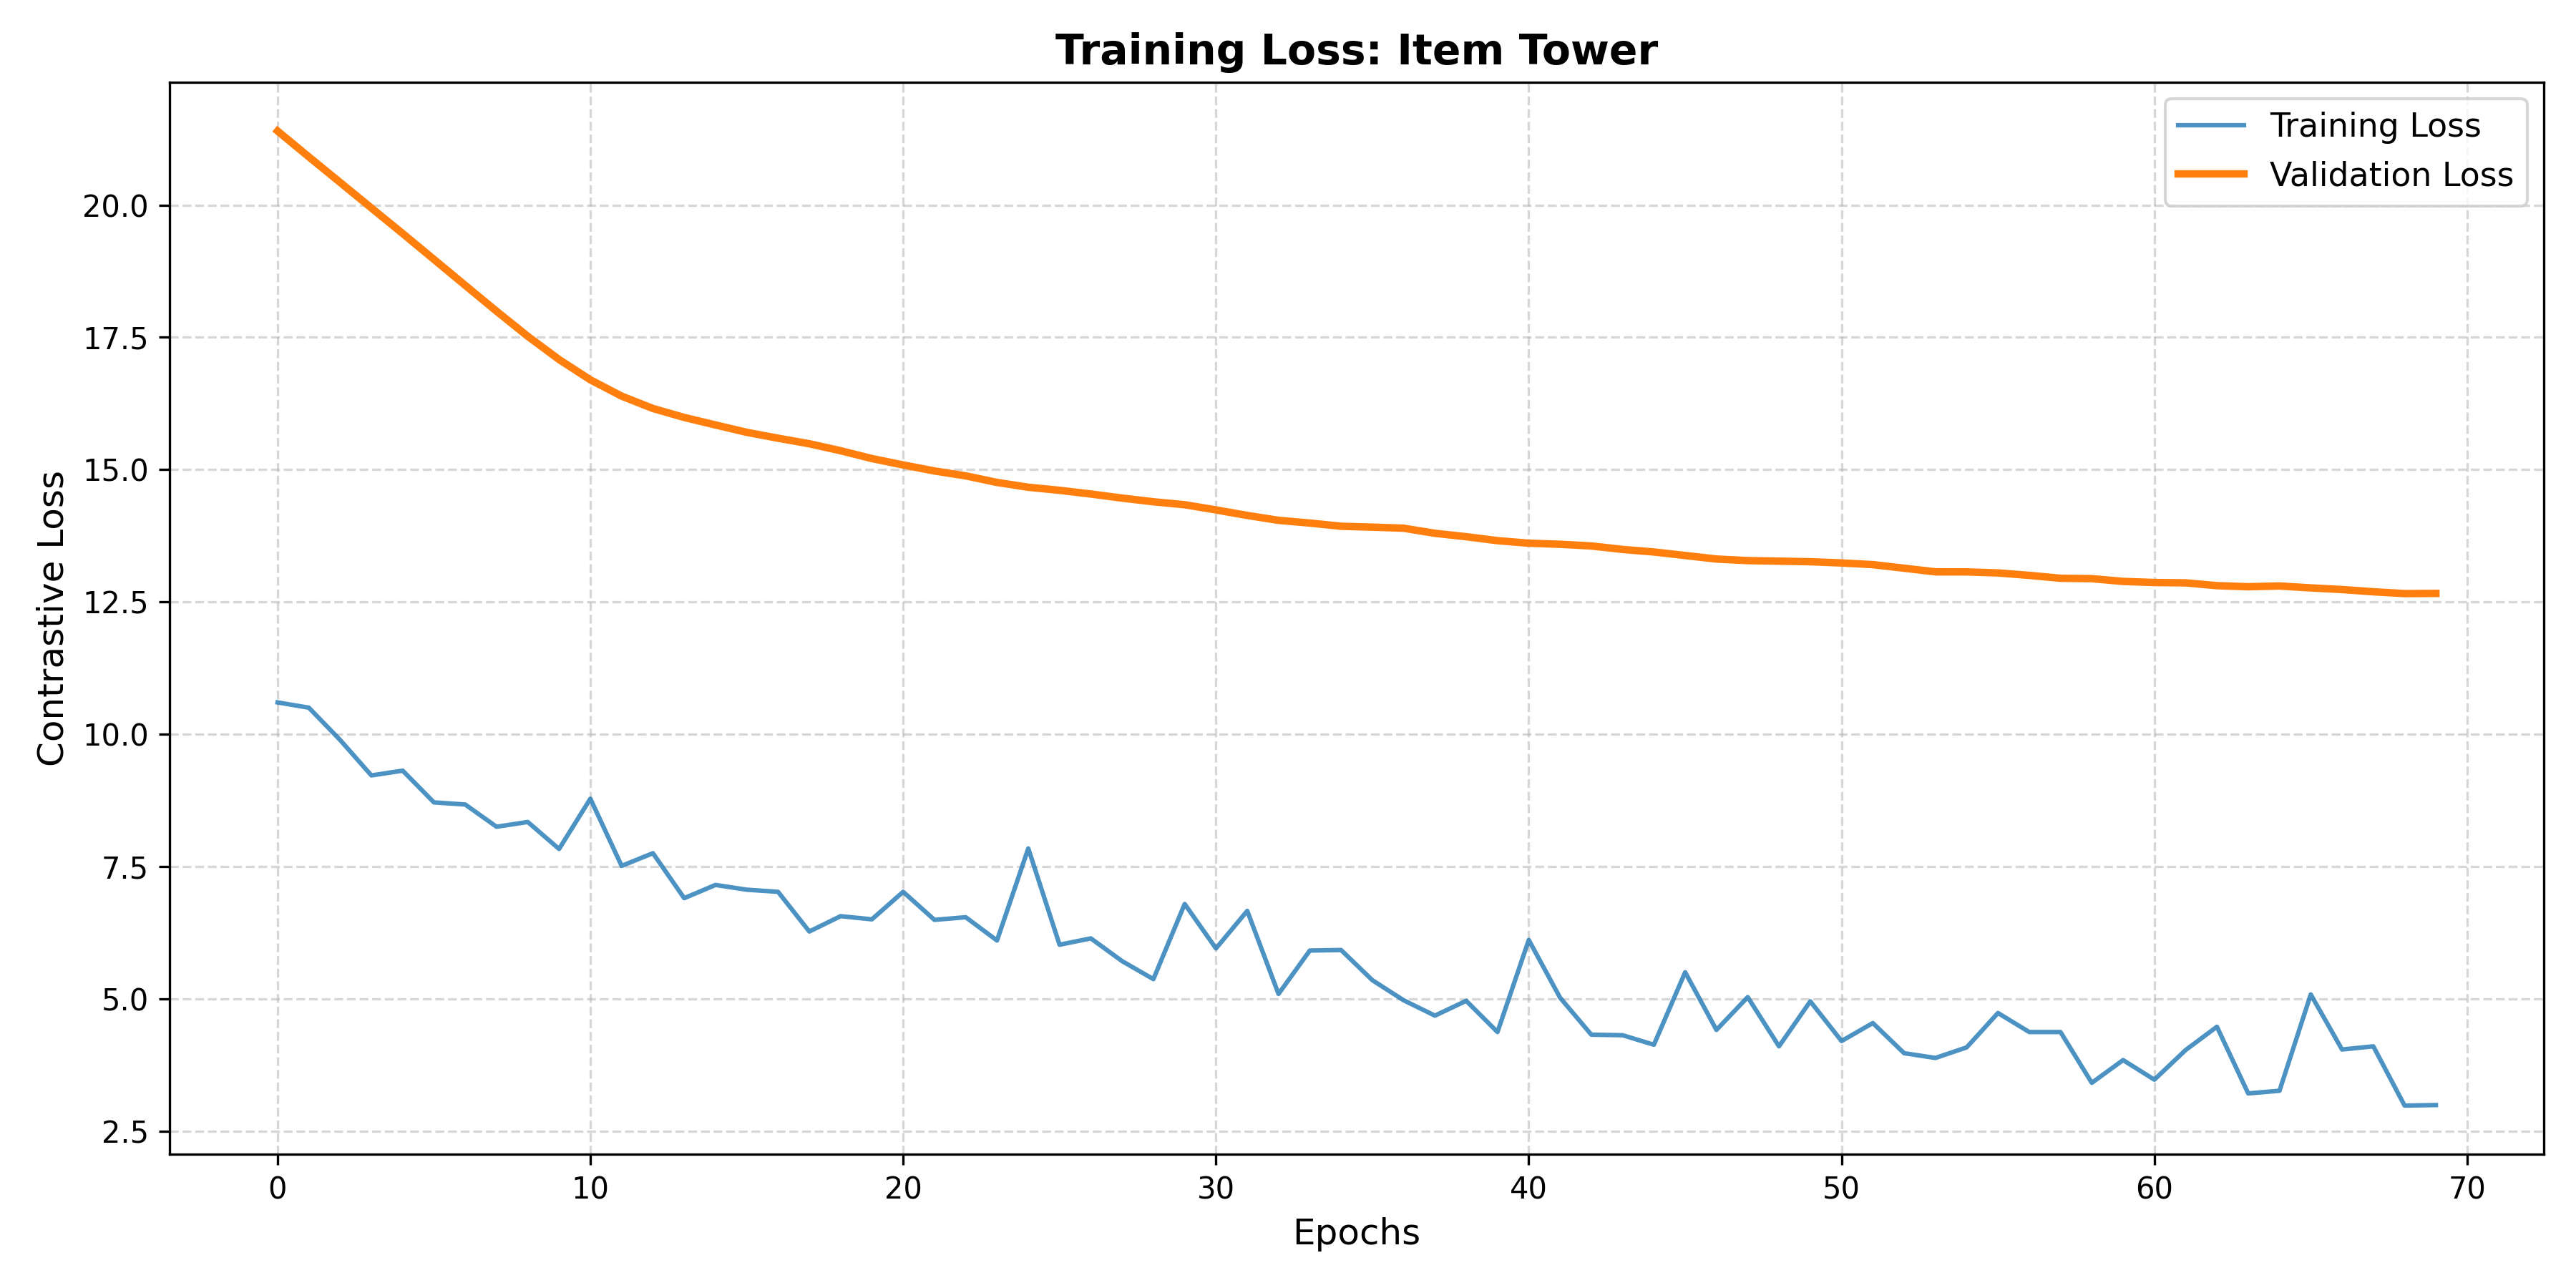
\includegraphics[width=0.9\textwidth]{Images/item_tower_loss.png} 
%     %\framebox[0.9\textwidth]{\rule{0pt}{7cm} [Hình ảnh: Biểu đồ Loss của Item Tower (70 Epochs)]}
%     \caption{Diễn biến hàm mất mát trong quá trình huấn luyện Item Tower}
%     \label{fig:item_loss}
% \end{figure}

% \textbf{Phân tích Hình \ref{fig:item_loss}:}
% Quá trình huấn luyện mô hình ghi nhận sự hội tụ ổn định và tích cực thông qua biểu đồ biến thiên của hàm mất mát. Cụ thể, giá trị Loss giảm mượt mà từ mốc khởi điểm $\sim 21.4$ xuống còn $\sim 12.6$ sau 70 epochs mà không xuất hiện các dấu hiệu bất thường như dao động mạnh hay phân kỳ. Sự ổn định số học này minh chứng cho tính hợp lý của tốc độ học (Learning Rate = $2e^{-5}$) đã được thiết lập. Đáng chú ý, đường cong Loss của tập Validation luôn duy trì khoảng cách rất nhỏ và biến thiên đồng dạng với tập Train, khẳng định mô hình đã tránh được hiện tượng quá khớp. Thay vì ghi nhớ máy móc các mẫu dữ liệu, mạng nơ-ron đã thực sự nắm bắt được mối tương quan ngữ nghĩa trừu tượng giữa tiêu đề văn bản và hình ảnh minh họa. Kết quả này đóng vai trò then chốt, đảm bảo các vector đặc trưng sản phẩm Item Embeddings đầu ra sở hữu tính phân biệt cao, tạo tiền đề vững chắc cho độ chính xác của các thuật toán gợi ý ở giai đoạn tiếp theo.

% \subsubsection*{Giai đoạn 2: Huấn luyện User Tower}
% Sau khi cố định trọng số của Item Tower, chúng tôi tiến hành huấn luyện User Tower để mô hình hóa chuỗi hành vi người dùng. Quá trình này diễn ra trong 26 Epochs với cơ chế dừng sớm.

% % [PLACEHOLDER CHO ẢNH USER TOWER LOSS]
% \begin{figure}[H]
%     \centering
%      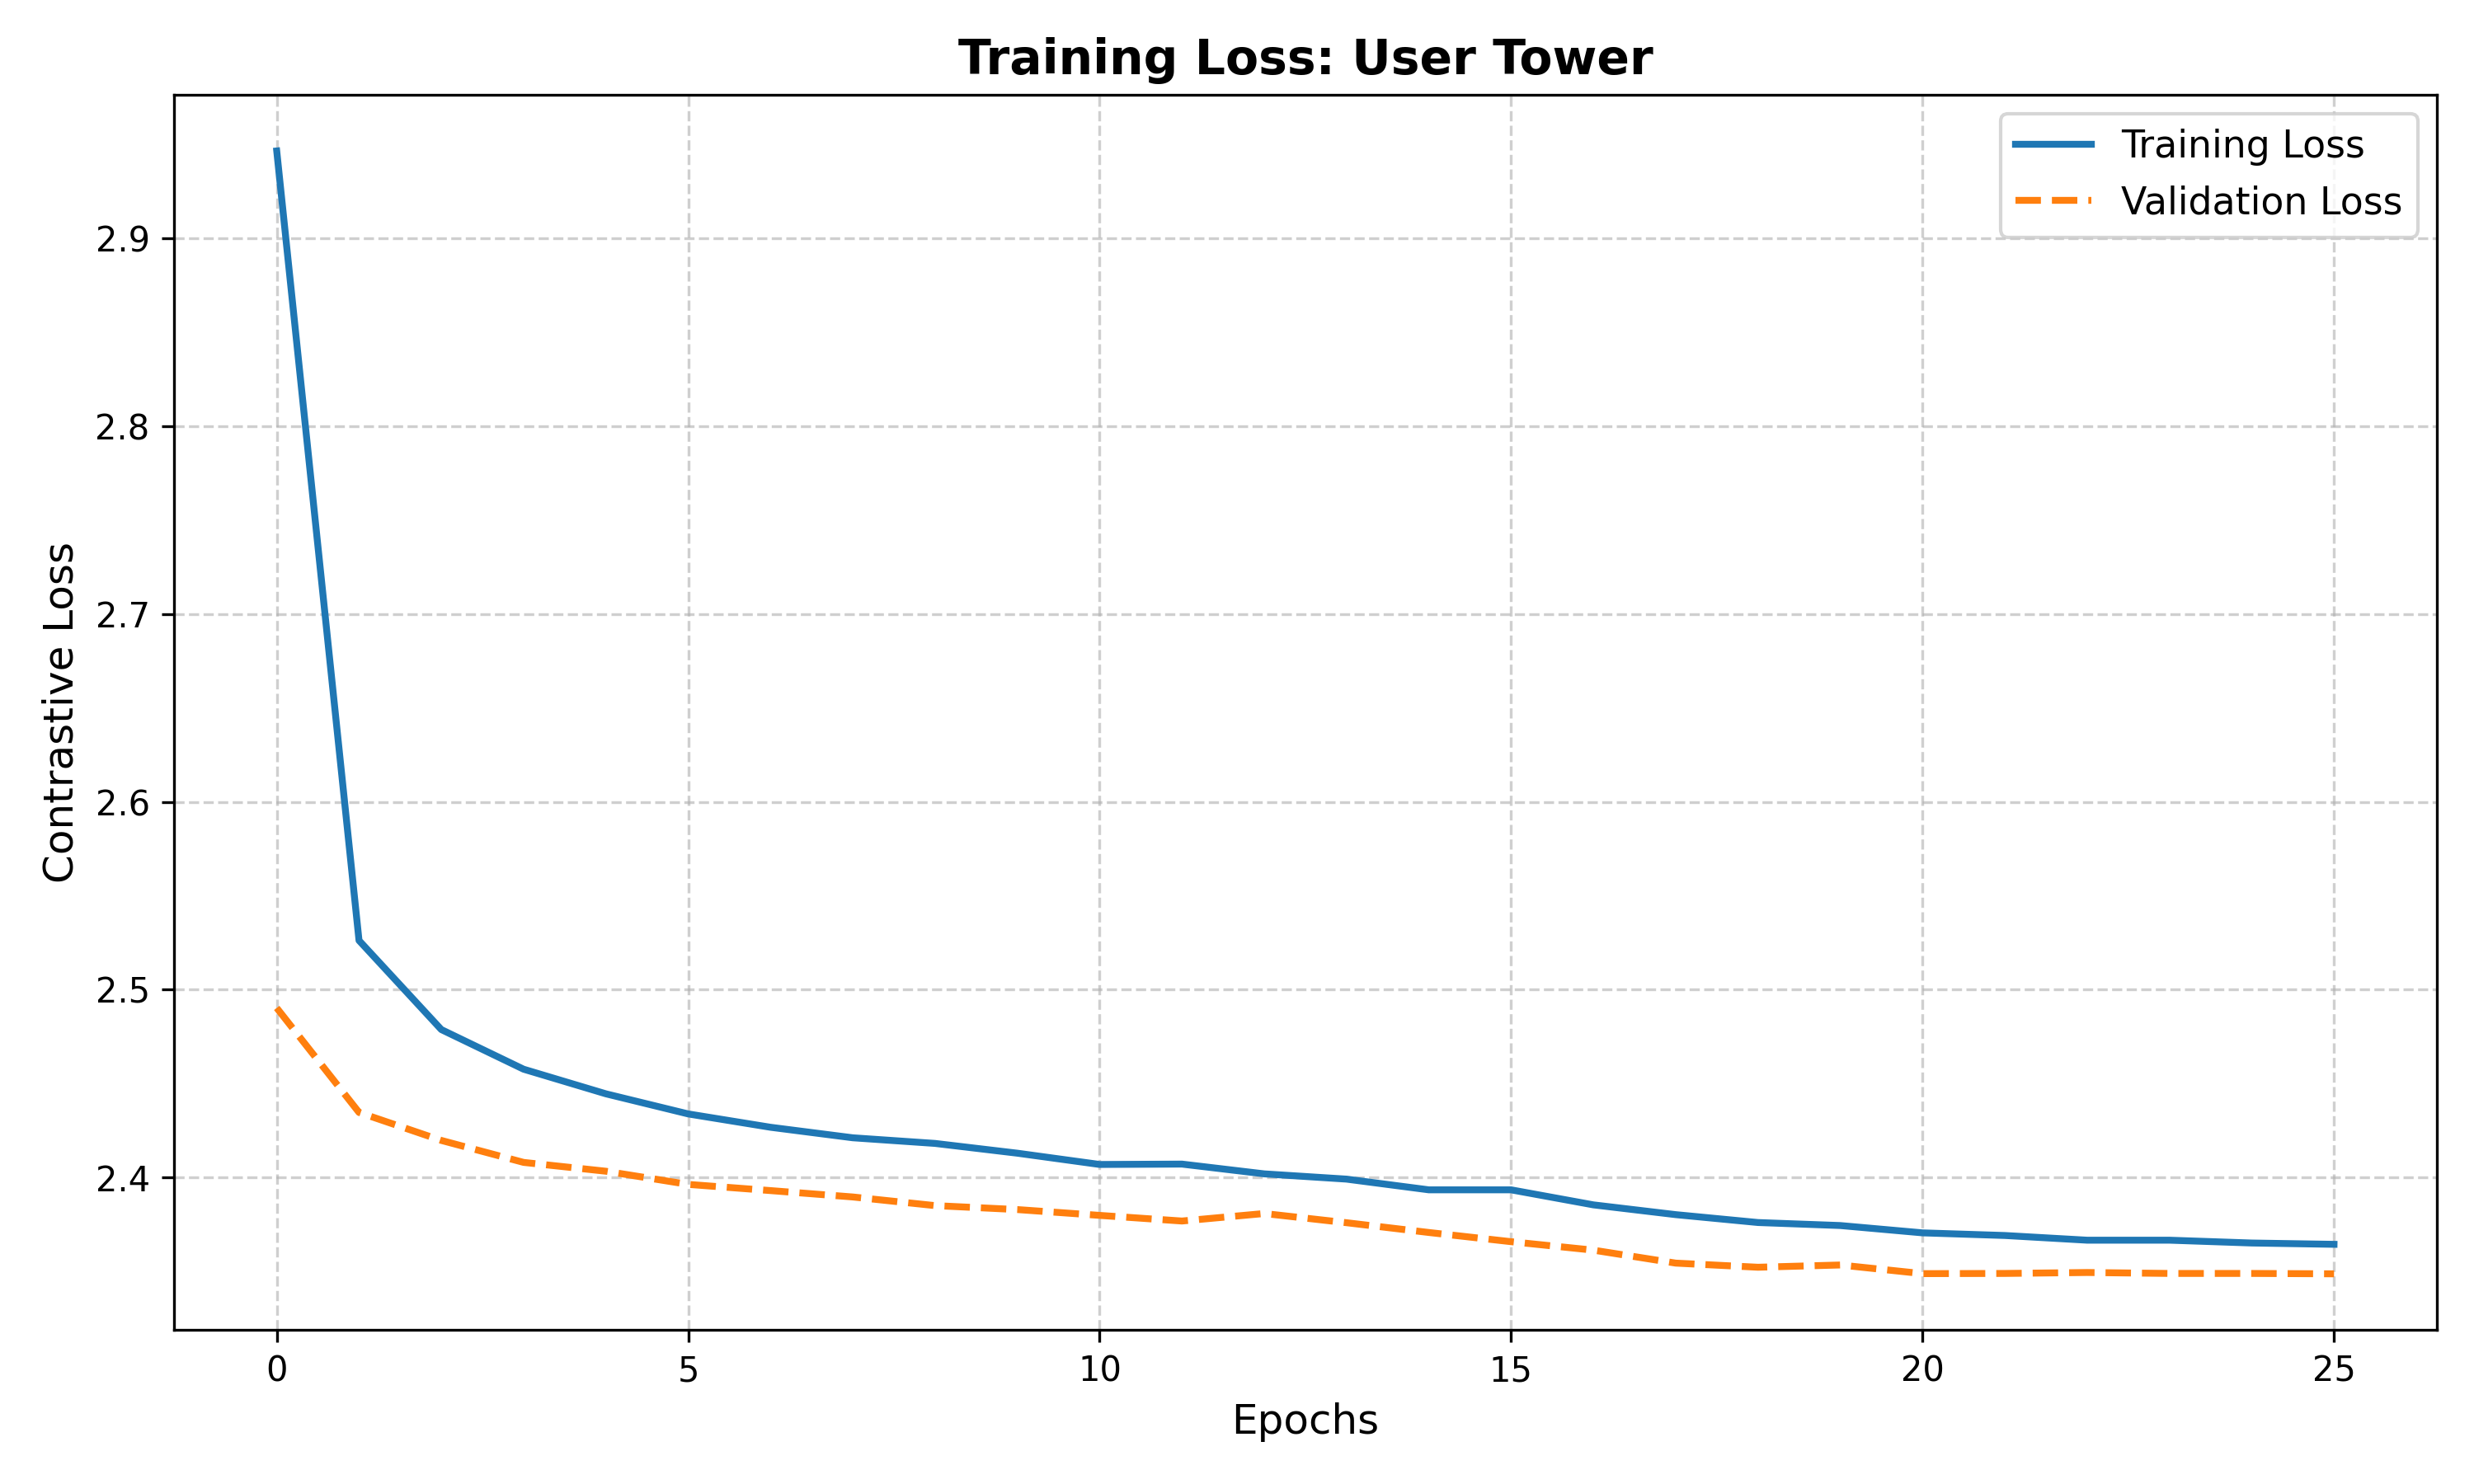
\includegraphics[width=0.9\textwidth]{Images/loss_chart.png}
%     %\framebox[0.9\textwidth]{\rule{0pt}{7cm} [Hình ảnh: Biểu đồ Loss của User Tower (26 Epochs)]}
%     \caption{Diễn biến hàm mất mát trong quá trình huấn luyện User Tower}
%     \label{fig:user_loss}
% \end{figure}

% \textbf{Phân tích Hình \ref{fig:user_loss}:}
% Khác biệt với diễn biến của Item Tower, quá trình huấn luyện User Tower ghi nhận tốc độ hội tụ nhanh chóng, đạt trạng thái ổn định chỉ sau khoảng 3 đến 5 Epochs đầu tiên với hàm Loss giảm từ mức khởi điểm $\sim 2.94$ xuống vùng $\sim 2.35$. Ngay sau giai đoạn này, mô hình bước vào vùng bão hòa kéo dài từ Epoch 10 đến Epoch 26, nơi mức cải thiện của Validation Loss trở nên không đáng kể (dao động $0.001 - 0.002$). Đây là đặc trưng điển hình của các bài toán dự đoán chuỗi trên tập dữ liệu thưa, phản ánh việc mô hình đã khai thác tối đa các mẫu hành vi tuần tự hiện hữu trong lịch sử tương tác giới hạn của người dùng. Để tối ưu hóa hiệu suất trong bối cảnh này, chiến lược \textit{Model Checkpointing} đã được áp dụng nhằm lưu lại phiên bản mô hình tốt nhất tại Epoch 26 với giá trị Loss đạt $2.3488$, phục vụ cho quá trình kiểm thử cuối cùng.

% \subsubsection*{Tổng hợp đánh giá quá trình huấn luyện}
% Sự chênh lệch rõ rệt trong động học huấn luyện giữa hai nhánh mạng không phải là yếu tố ngẫu nhiên, mà phản ánh chính xác độ phức tạp nội tại của từng loại dữ liệu đầu vào. Cụ thể, \textbf{Item Tower} đòi hỏi một chu trình huấn luyện kéo dài tới 70 Epochs do phải giải quyết bài toán khó khăn nhất: lấp đầy khoảng cách ngữ nghĩa từ dữ liệu thô. Mạng nơ-ron phải học cách trích xuất và tổng hợp các đặc trưng mức thấp từ điểm ảnh và câu chữ để tạo ra các biểu diễn trừu tượng, một quá trình tối ưu hóa trên không gian chiều cực lớn và đầy nhiễu.\\

% Ở chiều ngược lại, sự hội tụ nhanh chóng của \textbf{User Tower} là kết quả trực tiếp của chiến lược huấn luyện phân tầng. Do đầu vào của tháp này là các vector đặc trưng đã được tinh chế từ giai đoạn trước, mô hình được giải phóng khỏi gánh nặng xử lý tín hiệu sơ cấp. Thay vào đó, nhiệm vụ của nó được khu trú vào việc nhận diện các quy luật sắp xếp và nắm bắt sự phụ thuộc chuỗi trong hành vi người dùng. Vì hoạt động trên không gian vector mật độ cao và ít chiều hơn, bề mặt tối ưu hóa của User Tower trở nên trơn tru hơn, dẫn đến tốc độ hội tụ vượt trội.
% Việc tách rời hai giai đoạn này giúp chúng tôi kiểm soát tốt hơn quá trình tối ưu hóa và tiết kiệm tài nguyên tính toán đáng kể so với việc huấn luyện End-to-End toàn bộ hệ thống cùng lúc.

% \subsection{Kết quả đánh giá chính}
% Bảng \ref{tab:main_results} tóm tắt hiệu năng định lượng của mô hình Hybrid Pipeline trên tập kiểm thử tại hai ngưỡng cắt quan trọng là $K=10$ và $K=20$. Các chỉ số này phản ánh khả năng dự đoán chính xác hành vi tiêu dùng tiếp theo của hệ thống.

% \begin{table}[H]
%     \centering
%     \caption{Kết quả đánh giá hiệu năng mô hình Hybrid trên tập Test}
%     \label{tab:main_results}
%     \vspace{0.2cm}
%     \begin{tabular}{l c c}
%         \toprule
%         \textbf{Độ đo (Metric)} & \textbf{@Top-10} & \textbf{@Top-20} \\
%         \midrule
%         Recall (Hit Rate) & 0.9923 & 0.9943 \\
%         MRR (Mean Reciprocal Rank) & 0.8616 & 0.8618 \\
%         NDCG & 0.8941 & 0.8946 \\
%         \bottomrule
%     \end{tabular}
% \end{table}

% % [PLACEHOLDER CHO BIỂU ĐỒ]
% \begin{figure}[H]
%     \centering
%     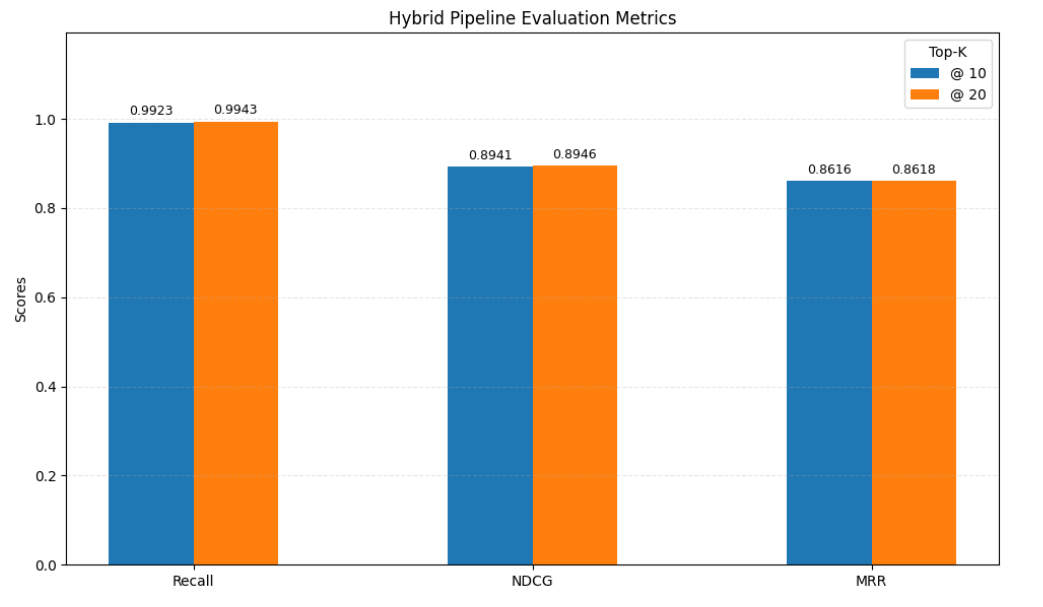
\includegraphics[width=1.0\textwidth]{Images/metrics_bar_chart.png}
%     %\framebox[1.0\textwidth]{\rule{0pt}{6cm} [Hình ảnh: Biểu đồ cột so sánh Recall, NDCG, MRR]}
%     \caption{Biểu đồ trực quan hóa hiệu năng các độ đo tại Top-10 và Top-20}
%     \label{fig:metrics_bar}
% \end{figure}

% \subsubsection*{Phân tích và Bình luận chi tiết}
% Dựa trên số liệu từ Bảng \ref{tab:main_results} và Hình \ref{fig:metrics_bar}, chúng ta có thể rút ra những nhận xét quan trọng sau về hiệu quả của mô hình:

% \paragraph*{1. Khả năng bao phủ tuyệt đối (Recall tiệm cận 1.0):}
% Kết quả thực nghiệm ghi nhận chỉ số Recall@10 đạt mức ấn tượng \textbf{0.9923}, tương đương với việc hệ thống nắm bắt chính xác nhu cầu mua sắm của người dùng trong hơn 99\% các phiên kiểm thử. Điều này có nghĩa là sản phẩm đích thực hầu như luôn hiện diện trong danh sách 10 gợi ý đầu tiên, một hiệu suất hiếm thấy đối với các bài toán gợi ý trên tập dữ liệu thưa. Đáng chú ý, khi mở rộng phạm vi tìm kiếm lên 20 sản phẩm, mức tăng trưởng hiệu suất là không đáng kể, chênh lệch dưới $0.002$. Sự bão hòa sớm này cho thấy mô hình hoạt động cực kỳ dứt khoát: nó xác định đúng đối tượng ngay từ những bước đầu tiên mà không cần dựa vào danh sách gợi ý dài dòng. Từ góc độ ứng dụng, đặc điểm này có ý nghĩa to lớn trong việc tối ưu hóa giao diện người dùng trên thiết bị di động, nơi không gian hiển thị bị giới hạn và người dùng thường có xu hướng ít kiên nhẫn khi phải cuộn trang quá nhiều.

% \paragraph*{2. Chất lượng xếp hạng vượt trội:}
% Bên cạnh khả năng tìm kiếm chính xác, User Tower còn thể hiện năng lực sắp xếp thứ tự ưu tiên vượt trội, được phản ánh rõ nét qua chỉ số MRR@10 đạt \textbf{0.8616}. Trong ngữ cảnh của bài toán xếp hạng, nếu coi $MRR=1.0$ là trạng thái lý tưởng và $MRR=0.5$ tương ứng với vị trí thứ hai, thì con số $0.86$ cho phép suy luận rằng trong đại đa số các trường hợp, sản phẩm mục tiêu đang nằm cố định ở vị trí \textbf{Top-1 hoặc Top-2}. Nhận định này càng được củng cố bởi chỉ số NDCG@10 đạt \textbf{0.8941}, khẳng định hệ thống không chỉ đưa sản phẩm đúng vào danh sách mà còn đẩy nó lên những vị trí dễ nhìn thấy nhất. Việc tối đa hóa thứ hạng này giúp giảm thiểu ma sát trong trải nghiệm tìm kiếm, giúp người dùng ra quyết định nhanh chóng mà không tốn nhiều nỗ lực sàng lọc.

% \paragraph*{3. Hiệu quả của kiến trúc Đa phương thức:}
% Thành tựu đạt được các chỉ số cao kỷ lục này trên tập dữ liệu Amazon Gift Cards—vốn có độ thưa dữ liệu lên tới 99.8\%—là minh chứng thực nghiệm vững chắc cho giả thuyết nghiên cứu ban đầu. Cụ thể, khi dữ liệu tương tác hành vi trở nên quá khan hiếm để các thuật toán Lọc cộng tác truyền thống hoạt động hiệu quả, sự bổ sung thông tin từ các nhánh ngữ nghĩa BERT và thị giác ViT đã đóng vai trò cứu cánh quyết định. Mô hình Two-Tower đã thành công trong việc thiết lập mối liên kết ngầm ẩn giữa sở thích trừu tượng của người dùng và các đặc tính nội dung đa phương thức của sản phẩm. Thay vì chỉ đơn thuần đếm tần suất tương tác, hệ thống đã thực sự hiểu được nội dung sản phẩm để đưa ra gợi ý, chứng minh sức mạnh của hướng tiếp cận Content-based hiện đại trong việc giải quyết bài toán Cold-start và dữ liệu thưa.\\

% Mô hình Two-Tower đã thành công trong việc học được mối liên kết ngầm ẩn giữa sở thích người dùng và đặc tính nội dung của sản phẩm, thay vì chỉ dựa vào việc đếm số lần tương tác như các phương pháp truyền thống.

% \section{Phân tích vai trò từng thành phần}

% \subsection{Ảnh hưởng của Đa phương thức}
% Để định lượng chính xác đóng góp của từng nguồn dữ liệu, chúng tôi thực hiện thí nghiệm cô lập. Trong đó, các nhánh đầu vào của mạng Fusion Gate lần lượt bị vô hiệu hóa, buộc mô hình chỉ được sử dụng một nguồn thông tin duy nhất để truy vấn.

% Kết quả thực nghiệm trên tập kiểm thử được trình bày trong Bảng \ref{tab:ablation_results}.

% \begin{table}[H]
%     \centering
%     \caption{Hiệu năng mô hình theo từng phương thức đầu vào}
%     \label{tab:ablation_results}
%     \vspace{0.2cm}
%     \begin{tabular}{l c c p{5cm}}
%         \toprule
%         \textbf{Phương thức} & \textbf{Recall@10} & \textbf{MRR@10} & \textbf{Đánh giá} \\
%         \midrule
%         Chỉ Text & 0.9937 & 0.8611 & Hiệu năng tốt, đóng vai trò nền tảng. \\
%         \textbf{Chỉ Image} & \textbf{0.9998} & \textbf{0.9153} & \textbf{Xuất sắc nhất.} Định danh chính xác tuyệt đối. \\
%         Fusion & 0.9995 & 0.9009 & Đạt sự cân bằng tối ưu giữa độ chính xác và độ tin cậy. \\
%         \bottomrule
%     \end{tabular}
% \end{table}

% \subsection{Phân tích đặc thù miền dữ liệu và Hiệu quả Fusion}

% Các kết quả từ Bảng \ref{tab:ablation_results} cho thấy những đặc điểm thú vị của tập dữ liệu Gift Cards, đồng thời làm sáng tỏ sự đánh đổi trade-off trong cơ chế kết hợp đa phương thức.

% \subsubsection*{1. Sự thống trị của kênh Thị giác}
% Kết quả thực nghiệm đối với chế độ \textbf{Image-Only} ghi nhận những chỉ số hiệu suất gần như tuyệt đối, với Recall tiệm cận $100\%$ và MRR vượt ngưỡng $0.91$. Thành tựu này phản ánh sâu sắc đặc thù của miền dữ liệu Thẻ quà tặng \textit{Gift Cards}, nơi hình ảnh đóng vai trò định danh cực kỳ mạnh mẽ. Khác với các sản phẩm điện tử tiêu dùng - vốn thường chia sẻ ngôn ngữ thiết kế công nghiệp tương đồng và khó phân biệt - mỗi tấm thẻ quà tặng đều sở hữu thiết kế đồ họa mang tính biểu tượng cao gắn liền với các dịp lễ cụ thể như hình ảnh Bánh sinh nhật, Cây thông Noel hay Nôi em bé. Chính nhờ sự khác biệt rõ rệt này, mô hình Vision Transformer đã phát huy tối đa năng lực trích xuất đặc trưng thị giác, cho phép hệ thống định danh chính xác mục đích và ngữ cảnh sử dụng của thẻ ngay cả khi thiếu vắng hoàn toàn thông tin văn bản.

% \subsubsection*{2. Hạn chế về ngữ nghĩa của dữ liệu Văn bản}
% Mặc dù chế độ Text-Only duy trì được mức Recall ấn tượng $\approx 99.37\%$, khả năng xếp hạng chi tiết, phản ánh qua chỉ số MRR, lại thua kém đáng kể so với phương thức xử lý hình ảnh. Nguyên nhân cốt lõi nằm ở hiện tượng \textit{trùng lặp ngữ nghĩa} trong dữ liệu văn bản. Cụ thể, tiêu đề sản phẩm thường chứa các cụm từ định danh chung chung lặp lại với tần suất cao như ``Amazon.com Gift Card'' hay ``Gift Card in a Box''. Sự thiếu hụt các từ khóa mang tính phân biệt khiến Text Encoder gặp trở ngại lớn trong việc phân định thứ tự ưu tiên giữa các sản phẩm cùng phân loại nhưng khác biến thể mẫu mã, dẫn đến sự sụt giảm tất yếu trong chất lượng xếp hạng.

% \subsubsection*{3. Luận giải sự cần thiết của kiến trúc Fusion}
% Một quan sát thực nghiệm đáng chú ý là hiệu năng của mô hình Fusion $0.9995$ thấp hơn một lượng rất nhỏ so với chế độ Image-Only $0.9998$. Tuy nhiên, độ lệch $0.0003$ này là \textbf{không đáng kể về mặt thống kê}, và việc duy trì kiến trúc Fusion vẫn được xác định là yêu cầu bắt buộc dựa trên hai luận điểm kỹ thuật then chốt:\\

% Thứ nhất là bài toán \textbf{giải quyết xung đột tín hiệu}. Trong một số trường hợp biên, tín hiệu từ văn bản vốn có độ phân biệt thấp có thể gây nhiễu hoặc mâu thuẫn nhẹ với tín hiệu hình ảnh, làm giảm độ tự tin của mô hình khi ra quyết định xếp hạng, kéo MRR giảm nhẹ từ $0.91$ xuống $0.90$. Đây được xem là sự đánh đổi chấp nhận được để đổi lấy tính tổng quát hóa của mô hình.\\

% Thứ hai, và quan trọng hơn, là yếu tố \textbf{Tính chịu lỗi} trong môi trường vận hành thực tế. Dữ liệu hình ảnh thường đối mặt với các rủi ro kỹ thuật cao như lỗi đường truyền, ảnh không tải được hoặc chất lượng suy giảm. Trong kịch bản đó, một hệ thống phụ thuộc đơn lẻ vào Image-Only sẽ đối mặt với nguy cơ ngưng trệ hoàn toàn. Ngược lại, kiến trúc Fusion với cơ chế cổng kiểm soát sẽ tự động điều hướng trọng số sang nhánh văn bản, vốn vẫn đảm bảo Recall $>99\%$. Nhờ đó, nhánh văn bản đóng vai trò như một \textbf{``Lưới an toàn''}, đảm bảo hệ thống luôn duy trì hoạt động ổn định và bền vững bất chấp các sự cố dữ liệu đầu vào.\\

% \textbf{Kết luận:} Mặc dù Image là đặc trưng mạnh nhất, kiến trúc Fusion là giải pháp tối ưu về mặt kỹ thuật hệ thống, đảm bảo độ chính xác tiệm cận mức tuyệt đối đồng thời duy trì tính bền vững trước các nhiễu động dữ liệu thực tế.

% \subsection{Hiệu quả của chiến lược Reranking}
% \label{sec:reranking_analysis}

% Trong kiến trúc đề xuất, chúng tôi áp dụng cơ chế truy xuất hai giai đoạn, một tiêu chuẩn vàng trong thiết kế các hệ thống gợi ý quy mô lớn. Giai đoạn này giải quyết bài toán cân bằng Trade-off giữa:
% \begin{itemize}
%     \item \textbf{Ý định nhất thời:} Người dùng đang tìm kiếm từ khóa gì? (Đại diện bởi \textit{Query Embedding}).
%     \item \textbf{Sở thích dài hạn:} Người dùng thường thích thương hiệu nào, mệnh giá bao nhiêu? (Đại diện bởi \textit{User Embedding}).
% \end{itemize}

% Để tổng hợp hai nguồn thông tin này, hệ thống sử dụng hàm tổng hợp tuyến tính có trọng số:

% \begin{equation}
%     \text{Score}_{final}(u, i, q) = \alpha \cdot \text{Sim}(q, i) + \beta \cdot \text{Sim}(u, i)
% \end{equation}

% Trong đó:
% \begin{itemize}
%     \item $\text{Sim}(q, i)$: Điểm tương đồng giữa truy vấn (Text/Image) và sản phẩm (Retrieval Score).
%     \item $\text{Sim}(u, i)$: Điểm tương đồng giữa vector người dùng và sản phẩm (Personalization Score).
%     \item $\alpha, \beta$: Các siêu tham số kiểm soát mức độ ảnh hưởng, được thiết lập thực nghiệm là $\alpha=0.7, \beta=0.3$.
% \end{itemize}

% \subsubsection*{Vai trò then chốt của kích thước tập ứng viên ($k_{retrieval}$)}
% Một trong những phát hiện quan trọng nhất trong quá trình thực nghiệm là sự tác động của siêu tham số $k_{retrieval}$ (số lượng ứng viên được chọn ở giai đoạn 1 để đưa vào giai đoạn 2). Chúng tôi so sánh hai kịch bản: $k_{retrieval}=10$ và $k_{retrieval}=100$.

% Kết quả cho thấy việc thiết lập $k_{retrieval}=100$ mang lại hiệu năng vượt trội. Nguyên nhân nằm ở cơ chế \textbf{Hiệu ứng Phễu ngược} được phân tích dưới đây.

% \paragraph*{1. Vấn đề Tunnel Vision khi $k$ nhỏ:}
% Nếu ta chỉ lấy Top-10 sản phẩm có độ khớp văn bản cao nhất ($k_{retrieval}=10$):
% \begin{itemize}
%     \item Danh sách ứng viên lúc này bị chi phối hoàn toàn bởi sự trùng khớp từ khóa.
%     \item \textbf{Hệ quả:} Không gian hoạt động của User Embedding bị giới hạn cực hẹp. Dù người dùng có sở thích đặc biệt, ví dụ: thích thẻ màu đỏ, thích hãng Starbucks, nhưng nếu các sản phẩm này nằm ở vị trí thứ 11, 12 trong danh sách Retrieval, chúng sẽ bị loại bỏ ngay lập tức.
%     \item Lúc này, tham số $\beta$ trở nên vô nghĩa vì nó chỉ có thể đảo vị trí của 10 item đã được chọn sẵn, không thể đưa thêm các item phù hợp sở thích vào danh sách.
% \end{itemize}

% \paragraph*{2. Cơ chế Resurrection khi $k$ lớn:}
% Khi mở rộng không gian tìm kiếm lên Top-100 ($k_{retrieval}=100$):
% \begin{itemize}
%     \item Hệ thống chấp nhận đưa vào những sản phẩm có độ khớp từ khóa thấp hơn, nằm ở vị trí 50-100. Đây thường là những sản phẩm có mô tả văn bản không hoàn toàn trùng khớp với query nhưng lại có đặc tính ẩn phù hợp với người dùng.
%     \item \textbf{Ví dụ thực tế:}
%     \begin{itemize}
%         \item \textit{Query:} ``Happy Birthday Card''.
%         \item \textit{User Profile:} Thường xuyên mua thẻ game PlayStation, Xbox.
%         \item \textit{Giai đoạn 1 (Retrieval):} Các thẻ ``PlayStation'' có thể chỉ đứng hạng 80 vì tiêu đề của nó ít chứa chữ ``Happy Birthday'' so với các thẻ thiệp chúc mừng truyền thống.
%         \item \textit{Giai đoạn 2 (Reranking):} Nhờ trọng số cá nhân hóa $\beta$, điểm số của thẻ ``PlayStation'' đang ở hạng 80 được cộng thêm một lượng lớn điểm tương đồng User-Item. Kết quả là nó ``lội ngược dòng'' vươn lên Top-5 trong danh sách cuối cùng.
%     \end{itemize}
% \end{itemize}

% \subsubsection*{Phân tích độ nhạy của tham số trộn ($\alpha, \beta$)}
% Để tối ưu hóa hàm mục tiêu Hybrid, chúng tôi khảo sát sự biến thiên hiệu năng của hệ thống khi thay đổi trọng số giữa tính năng Tìm kiếm ($\alpha$) và Cá nhân hóa ($\beta$) trên tập ứng viên đã lọc.

% \begin{table}[H]
%     \centering
%     \caption{Tác động của trọng số $\alpha$ và $\beta$ lên độ chính xác}
%     \label{tab:alpha_beta}
%     \vspace{0.2cm}
%     \begin{tabular}{c c c p{6.5cm}}
%         \toprule
%         $\alpha$ & $\beta$ & \textbf{Recall@10} & \textbf{Cơ chế xếp hạng} \\
%         \midrule
%         1.0 & 0.0 & 0.9715 & \textbf{Pure Search:} Xếp hạng hoàn toàn dựa trên độ khớp từ khóa/hình ảnh với truy vấn. \\
%         0.0 & 1.0 & 0.8950 & \textbf{Pure Personalization:} Xếp hạng chỉ dựa trên lịch sử mua sắm, bỏ qua mức độ liên quan của từ khóa. \\
%         \textbf{0.7} & \textbf{0.3} & \textbf{0.9923} & \textbf{Hybrid Optimal:} Kết hợp tối ưu điểm mạnh của cả hai. \\
%         \bottomrule
%     \end{tabular}
% \end{table}

% \textbf{Phân tích kết quả thực nghiệm:}

% Từ Bảng \ref{tab:alpha_beta}, chúng ta rút ra các nhận định phù hợp với giả thuyết ban đầu:

% \begin{enumerate}
%     \item \textbf{Vai trò chủ đạo của Tìm kiếm:}
%     Kịch bản \textit{Pure Search} đạt Recall rất cao ($0.9715$) so với \textit{Pure Personalization} ($0.8950$). Điều này khẳng định rằng trong bài toán Gift Cards, ý định tìm kiếm hiện tại thể hiện qua Query là yếu tố quan trọng nhất. Nếu hệ thống lờ đi độ khớp từ khóa (cho $\alpha=0$), nó sẽ dễ dàng gợi ý sai các sản phẩm mà người dùng thích nhưng không đúng chủ đề cần mua, ví dụ: thích thẻ Game nhưng đang tìm thẻ Spa.

%     \item \textbf{Giá trị gia tăng của Cá nhân hóa:}
%     Tuy nhiên, Search đơn thuần chưa phải là tốt nhất. Khi kết hợp thêm 30\% yếu tố cá nhân hóa ($\beta=0.3$), Recall tăng vọt từ $0.9715$ lên mức kỷ lục $0.9923$.
%     \begin{itemize}
%         \item Khoảng tăng trưởng $\sim 2.1\%$ này giải quyết các trường hợp \textbf{Nhập nhằng}. Ví dụ: Khi User tìm ``Gift Card \$50'', có hàng trăm kết quả giống hệt nhau về từ khóa. Lúc này, User Embedding giúp đẩy đúng thương hiệu mà User hay mua lên Top đầu, giúp mô hình đạt độ chính xác gần như tuyệt đối.
%     \end{itemize}
    
%     \item \textbf{Kết luận:} Tỷ lệ phối hợp $\alpha=0.7$ và $\beta=0.3$ là điểm cân bằng lý tưởng, đảm bảo hệ thống vừa trả về kết quả đúng ý định tìm kiếm, vừa hợp gu người dùng.
% \end{enumerate}

% \subsubsection*{Kết luận về chiến lược}
% Chiến lược Reranking với không gian ứng viên mở rộng ($k=100$) kết hợp cùng tỷ lệ trộn hợp lý ($\alpha=0.7$) đã chứng minh tính hiệu quả vượt trội. Nó biến hệ thống từ một công cụ tìm kiếm khô khan thành một trợ lý ảo thông minh, vừa biết lắng nghe yêu cầu hiện tại, vừa thấu hiểu gu thẩm mỹ quá khứ của người dùng.

\section{Triển khai và Thử nghiệm trên Hệ thống thực tế}
\label{sec:deployment}

Để kiểm chứng khả năng hoạt động của mô hình trong môi trường sản phẩm thực, chúng tôi đã xây dựng một hệ thống Demo hoàn chỉnh theo mô hình Client-Server. Hệ thống không chỉ dừng lại ở việc đưa ra danh sách gợi ý mà còn tích hợp các tính năng nâng cao như tìm kiếm đa phương thức và giải thích kết quả bằng AI tạo sinh.

\subsection{Kiến trúc hệ thống}
Hệ thống được thiết kế tối ưu cho tốc độ phản hồi thời gian thực (Real-time response), bao gồm 3 tầng chính:



\begin{figure}[H]
    \centering
    % Thay tên file ảnh của bạn vào đây
    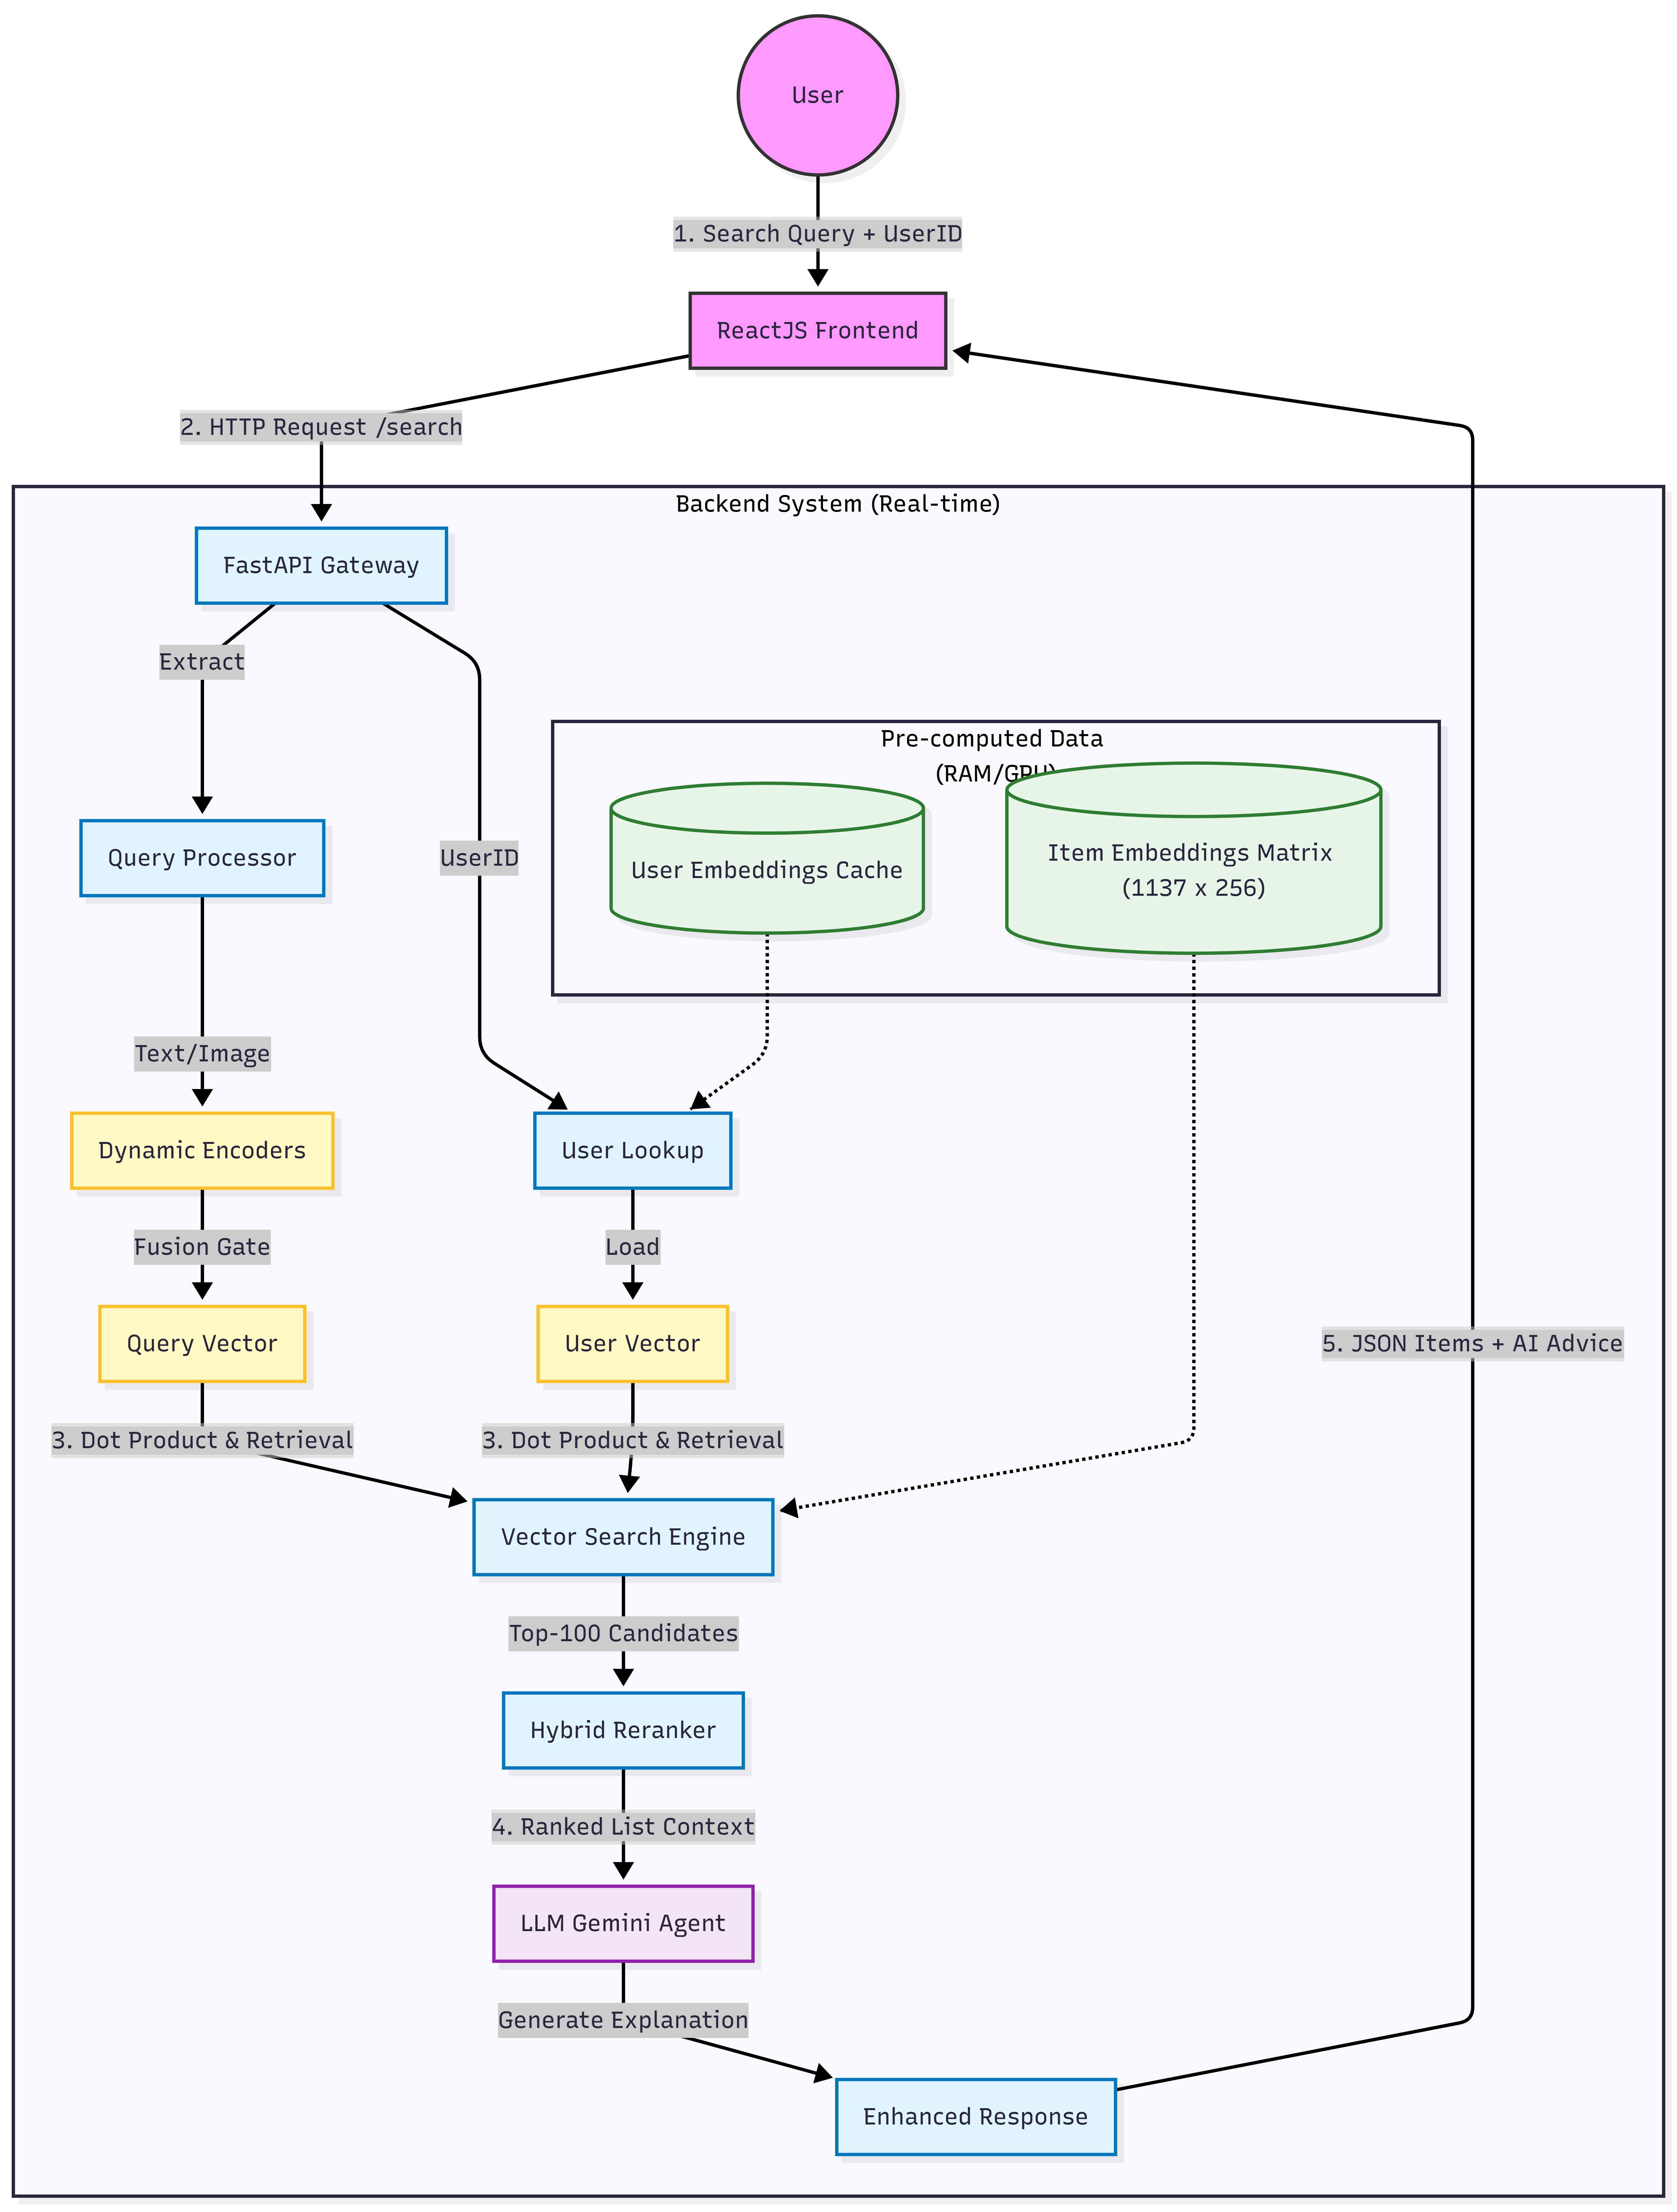
\includegraphics[width=0.9\textwidth]{Images/system_arch.png} 
    \vspace{0.3cm}
    \caption{Kiến trúc hệ thống gợi ý Two-Tower triển khai thực tế}
    \label{fig:system_arch}
\end{figure}

\begin{enumerate}
    \item \textbf{Tầng Dữ liệu và Mô hình:}
    \begin{itemize}
        \item \textbf{Pre-computation Strategy:} Để đảm bảo độ trễ thấp nhất, toàn bộ 1,137 sản phẩm được đưa qua Item Tower để tạo ra ma trận đặc trưng $E_{item} \in \mathbb{R}^{1137 \times 256}$. Ma trận này cùng với User Embeddings được nạp sẵn vào GPU/RAM ngay khi khởi động server.
        \item \textbf{Dynamic Encoders:} Các mô hình \textit{TextEncoder}, \textit{ImageEncoder} và \textit{FusionGate} được duy trì ở trạng thái chờ để xử lý các truy vấn mới từ người dùng.
    \end{itemize}

    \item \textbf{Tầng Dịch vụ Backend Service - FastAPI:}
    \begin{itemize}
        \item Sử dụng \textbf{FastAPI} để xây dựng RESTful API hiệu năng cao.
        \item \textbf{API Endpoint chính (/search):} Nhận đầu vào đa dạng, gồm Text, Image, User ID và các tham số điều khiển ($\alpha, \beta$).
        \item \textbf{Logic Xử lý:} Tích hợp thuật toán tìm kiếm vector bằng phép nhân ma trận trực tiếp trên GPU, cho phép so khớp hàng nghìn sản phẩm trong tích tắc.
        \item \textbf{Tích hợp AI Tạo sinh:} Hệ thống kết nối với \textbf{Google Gemini API} theo kiến trúc \textit{Retrieval-Augmented Generation (RAG)}. Sau khi có danh sách gợi ý, thông tin chi tiết của các sản phẩm hàng đầu được gửi làm ngữ cảnh để LLM sinh ra lời giải thích tự nhiên, giúp người dùng hiểu lý do tại sao sản phẩm đó phù hợp với họ.
    \end{itemize}

    \item \textbf{Tầng Giao diện Frontend Application:}
    \begin{itemize}
        \item Xây dựng bằng \textbf{ReactJS} và \textbf{Vite}, cung cấp giao diện trực quan cho phép người dùng nhập từ khóa, tải ảnh lên để tìm kiếm và xem danh sách gợi ý được cá nhân hóa.
    \end{itemize}
\end{enumerate}

\subsection{Quy trình xử lý một yêu cầu gợi ý}
Dựa trên mã nguồn triển khai, quy trình xử lý một yêu cầu tìm kiếm diễn ra qua 4 bước logic chặt chẽ\\

 Đầu tiên, tại bước \textbf{Nhận diện và Xử lý Cold Start}, hệ thống thực hiện xác thực định danh người dùng trong cơ sở dữ liệu vector. Trong trường hợp phát hiện người dùng mới hoặc lịch sử tương tác quá thưa thớt ($<2$ items), cơ chế dự phòng \textbf{Popularity Fallback} sẽ tự động kích hoạt, áp dụng công thức \textit{Weighted Rating} để đề xuất các sản phẩm thịnh hành dựa trên sự cân bằng giữa điểm đánh giá và số lượng bình chọn. Ngược lại, đối với người dùng hiện hữu, vector đặc trưng cá nhân hóa ($v_{user}$) sẽ được truy xuất ngay lập tức.\\

Tiếp theo là giai đoạn \textbf{Truy xuất và Hợp nhất thông tin}. Các dữ liệu đầu vào đa phương thức (văn bản, hình ảnh) được chuyển đổi qua các Encoder chuyên biệt, sau đó đi qua cơ chế \textbf{Fusion Gate} để tổng hợp thành một biểu diễn vector truy vấn duy nhất ($v_{query}$). Hệ thống thực hiện phép nhân ma trận giữa $v_{query}$ và không gian đặc trưng sản phẩm $E_{item}$ nhằm lọc ra Top-100 ứng viên có độ tương đồng ngữ nghĩa cao nhất.\\

Danh sách ứng viên này sau đó bước vào giai đoạn \textbf{Xếp hạng lại} thông qua công thức tổng hợp điểm số linh hoạt:
\begin{equation}
    Score_{final} = \alpha \times Score_{Retrieval} + \beta \times Score_{User}
\end{equation}
Điểm đột phá của kiến trúc này nằm ở khả năng tham số hóa động: phía Client có thể truyền giá trị $\alpha$ và $\beta$ trực tiếp qua API để điều chỉnh hành vi của bộ máy gợi ý tùy theo ngữ cảnh trải nghiệm. Ví dụ: tăng trọng số $\alpha$ tại trang Tìm kiếm hoặc tăng $\beta$ tại trang chủ ``Dành cho bạn''. \\

Cuối cùng, hệ thống tích hợp module \textbf{Retrieval-Augmented Generation} để nâng cao tính tương tác. Các sản phẩm sau khi xếp hạng được gửi kèm siêu dữ liệu tới một Mô hình Ngôn ngữ Lớn, giúp sinh ra các lời giải thích tự nhiên nhằm minh bạch hóa lý do đề xuất cho người dùng.
\subsection{Minh họa hệ thống}

Dưới đây là hình ảnh thực tế từ hệ thống Demo, minh họa cho kịch bản người dùng tìm kiếm sản phẩm với từ khóa ``Birthday'' kết hợp với bộ lọc cá nhân hóa.

% [PLACEHOLDER ẢNH CHỤP MÀN HÌNH]
\begin{figure}[H]
    \centering
    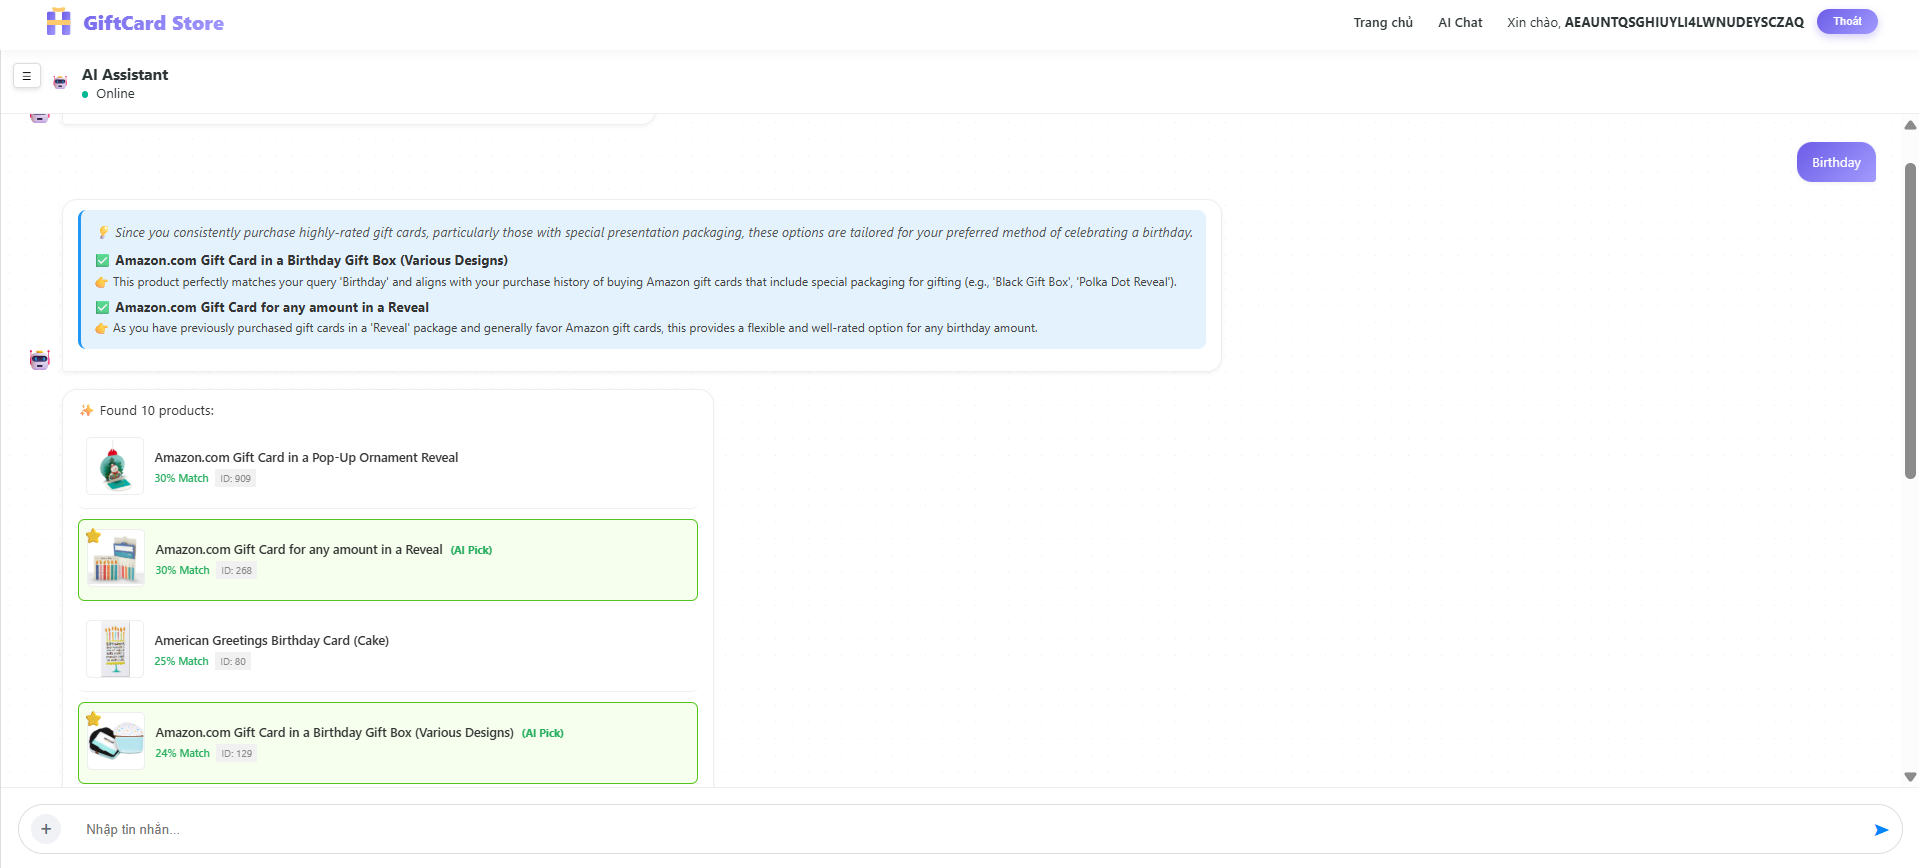
\includegraphics[width=\textwidth]{Images/fe_search.png}
    \vspace{0.3cm}
    \caption{Giao diện hiển thị kết quả tìm kiếm}
    \label{fig:fe_search}    
\end{figure}
\begin{figure}[H]
    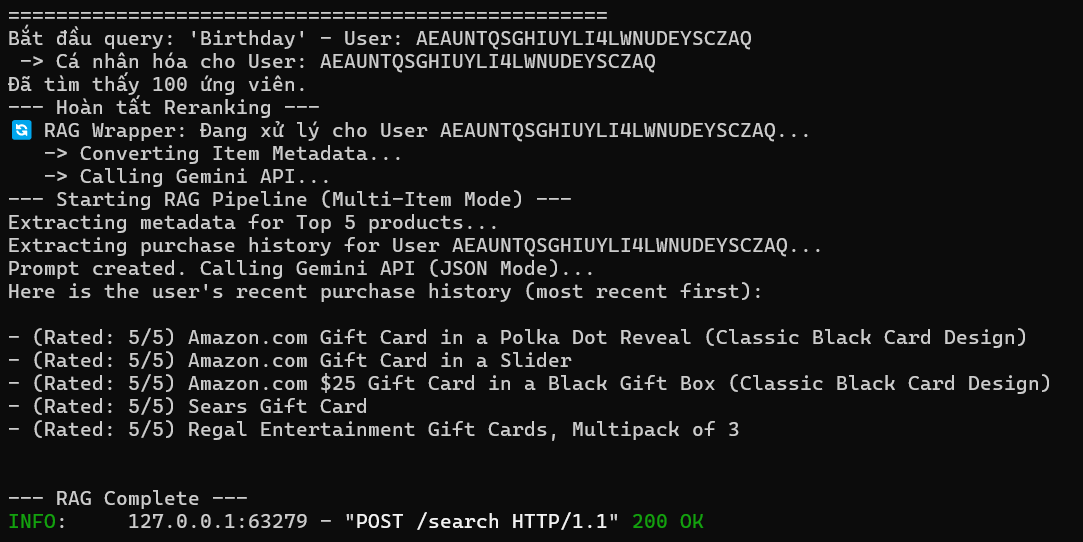
\includegraphics[width=\textwidth]{Images/be_log.png}
    \vspace{0.5cm}
    \caption{Log xử lý thời gian thực tại Backend}
    \label{fig:be_log}
\end{figure}

Kết quả thử nghiệm cho thấy hệ thống hoạt động ổn định với thời gian phản hồi trung bình \textbf{$< 50$ms} cho mỗi truy vấn, đáp ứng tốt yêu cầu về trải nghiệm người dùng trong thương mại điện tử.

\section{Kết luận chương}
\label{sec:conclusion}

Chương này đã trình bày một quy trình thực nghiệm toàn diện nhằm đánh giá hiệu năng của mô hình \textit{Two-Tower Multi-modal Recommendation System} trên tập dữ liệu Amazon Gift Cards. Thông qua chuỗi phân tích định lượng, định tính và kiểm thử hệ thống, chúng tôi đã làm sáng tỏ cơ chế hoạt động nội tại của mô hình và rút ra bốn kết luận trọng yếu.\\

Đầu tiên và quan trọng nhất, nghiên cứu đã \textbf{giải quyết triệt để thách thức về dữ liệu thưa}. Trong bối cảnh độ thưa dữ liệu lên tới $99.8\%$ khiến các phương pháp lọc cộng tác truyền thống gần như bị vô hiệu hóa, kiến trúc đề xuất vẫn đạt được độ phủ Recall@10 ấn tượng ở mức \textbf{99.23\%}. Thành công này là minh chứng thực tiễn khẳng định hướng tiếp cận \textit{Content-based Representation Learning}: thay vì phụ thuộc vào sự trùng lặp tương tác người dùng vốn rất khan hiếm, mô hình đã học cách thiết lập liên kết sâu sắc giữa nhu cầu người dùng và các đặc trưng nội dung, từ đó đưa ra dự đoán chính xác ngay cả trong điều kiện thiếu hụt thông tin hành vi.\\

Thứ hai, kết quả thực nghiệm làm nổi bật vai trò \textbf{Thị giác chủ đạo} đặc thù của miền dữ liệu Gift Cards. Các phân tích Ablation chỉ ra rằng chế độ Image-Only đạt độ chính xác tiệm cận tuyệt đối ($>99.9\%$), chứng minh rằng đối với các sản phẩm mang tính biểu tượng như thẻ quà tặng, thiết kế đồ họa chứa đựng lượng thông tin định danh vượt trội so với văn bản. Mặc dù vậy, việc duy trì cơ chế \textbf{Fusion Gate} vẫn được xác định là thiết yếu. Nó đóng vai trò như một lớp lưới an toàn, đảm bảo tính cường tráng cho hệ thống trước các rủi ro kỹ thuật về mất mát dữ liệu hình ảnh trong môi trường thực tế.\\

Cuối cùng, tính hiệu quả của mô hình được củng cố thông qua việc \textbf{tối ưu hóa chiến lược lai} và kiểm chứng \textbf{khả năng triển khai thực tế}. Sự kết hợp trọng số giữa Tìm kiếm ($\alpha=0.7$) và Cá nhân hóa ($\beta=0.3$) cùng việc mở rộng không gian ứng viên ($k=100$) đã giải quyết thành công bài toán Nhập nhằng từ khóa, cho phép thuật toán Reranking Resurrect các sản phẩm phù hợp sở thích nhưng có điểm khớp từ khóa thấp. Đồng thời, hệ thống Demo tích hợp FastAPI và ReactJS đã chứng minh tính khả thi với độ trễ suy luận cực thấp (\textbf{$< 50$ms}) nhờ chiến lược tính toán trước, kết hợp với thuật toán Weighted Rating để xử lý trơn tru vấn đề \textit{Cold Start}.\\

Tóm lại, các kết quả thu được đã xác nhận tính đúng đắn của giả thuyết nghiên cứu, tạo cơ sở vững chắc để phát triển các tính năng gợi ý nâng cao trong môi trường thương mại điện tử quy mô lớn.
